\section{空间离散方法}

\subsection{有限差分方法}
{\color{red}\begin{center}
    谭力玮
\end{center}}

\subsection{谱方法}          

    谱方法起源于1820年,Navier用双重三角函数来求解长方形薄板问题。但是,很长一段时间,谱方法并没有得到广泛应用,主要因为计算量过大,直到1965年快速Fourier变换的出现,谱方法的研究又得以快速发展,谱方法与差分法和有限元法有较大的不同,主要体现在谱方法的检验函数被取为无穷可微的整体函数。根据检验函数的不同,谱方法可分为Galer谱方法、Tau方法和配点法,其中,Galerkin谱方法可简称为谱方法,配点法又称为拟谱方法。如果按边值条件是否有周期性,又可分为Fourier谱方法(周期情形)、Chebyshev谱方法、Legendre谱方法和Hermite谱方法等,它们分别以三角函数、Chebyshev多项式、Legendre多项式和Hermite多项式为基函数来研究问题。

\subsubsection{Fourier谱方法}                           
{\color{red}\begin{center}             
     刘双
\end{center}}                                                                                                      
                                                                                                                                                                                                                                                                                                                                                                                                                                                                                                                                                                                                                                                                                          \textbf{连续和离散傅里叶变换}
                                                                                                                                                                                                                                                                                                                                                                                                                                                                                                                                                                                                                                                                                          
    这部分致力于简单回顾傅里叶级数和傅里叶变换的性质。主要关注点放在离散傅里叶变换和傅里叶微分技术上,它们在傅里叶谱方法中发挥着重要的作用。
        
\begin{itemize}
  \item  \textbf{连续傅里叶级数}
\end{itemize}        

    我们用下式来表示复指数    
\begin{equation*}
    E_k(x) := e^{ikx} = \cos kx + i\sin kx = (\cos x + i\sin x)^k, \   k \in \mathbb{Z},x \in \mathbb{R},
\end{equation*}    
    其中$i = \sqrt{-1}$。集合$\{ e^{ikx}:k \in \mathbb{Z} \}$构成复希尔伯特空间$L^2 (0,2\pi)$上的一个完全正交组,其中配有内积和范数    
\begin{equation*}
    (u,v) = \dfrac{1}{2\pi} \int_0^{2\pi} u(x)\bar{v}(x)dx, \  
    \| u \| = \sqrt{(u,u)},
\end{equation*}    
    其中$\bar{v}$是$v$的共轭复数。$\{ E_k:k \in \mathbb{Z}\}$的正交性如下    
\begin{equation}
    (E_k,E_m) = \dfrac{1}{2\pi} \int_0^{2\pi} e^{i(k - m)x} dx = \delta_{km}
\label{6.2.1}    
\end{equation}    
    其中$\delta_{km}$表示克罗内克符号。
    
    对任意复值函数$u \in L^2(0,2\pi)$,它的傅里叶级数定义为    
\begin{equation}
    u(x) \thicksim \mathcal{F} (u)(x) := \sum_{k = -\infty}^{\infty} \hat{u}_ke^{ikx} ,
    \label{6.2.2}
\end{equation}    
    其中傅里叶系数由下式给出    
\begin{equation}
    \hat{u}_k = (u,e^{ikx}) = \dfrac{1}{2\pi} \int_0^{2\pi} u(x)e^{-ikx} dx .
    \label{6.2.3}
\end{equation}    

    如果$u$是实值函数,显然它的傅里叶系数满足    
\begin{equation}
    \hat{u}_{-k} = \bar{\hat{u}}_k, \   k \in \mathbb{Z},
    \label{6.2.4}
\end{equation}    
    由此易知此时$\hat{u}_0$是实数。
    
    事实上,傅里叶级数可以定义为通常$(0,2\pi)$上绝对可积函数,傅里叶展开的收敛性理论在傅里叶分析中已经有过严谨且彻底的研究(例如参见Zygmund (2002), Stein and Shakarchi (2003))。我们知道,对于任意$u \in L^2(0.2\pi)$, 其截断傅里叶级数$\mathcal{F}_N(u) := \sum_{|k| \leq N} \hat{u}_k e^{ikx}$在$L^2$意义下收敛至$u$,且有Parseval恒等式:   
\begin{equation}
    \| u \|^2 = \sum_{k = -\infty}^{\infty} |\hat{u}_k|^2.
    \label{6.2.5}
\end{equation}       

    如果$u$在$[0,2\pi]$上是连续的、周期的和有界变差的,那么$\mathcal{F}_N(u)$一致收敛于$u$。
    
    注意到截断傅里叶级数也可以用卷积的形式表示,即    
\begin{equation}
    \mathcal{F}_N(u)(x) = (\mathcal{D}_N * u)(x) = \dfrac{1}{2\pi} \int_0^{2\pi} \mathcal{D}_N(x - t)u(t) dt,
\label{6.2.6}
\end{equation}    
    其中$\mathcal{D}_N$是已知的狄利克雷内核    
\begin{equation}
    \mathcal{D}_N(x) := \sum_{k = -N}^N e^{ikx} = 1 + 2\sum_{k = 1}^N \cos kx = \dfrac{\sin ((N + 1/2)x)}{\sin (x/2)}.
    \label{6.2.7}
\end{equation}    

    有时用三角函数表示傅里叶级数较方便:   
\begin{equation}
    u(x) \thicksim \mathcal{T}(u)(x) = \dfrac{a_0}{2} + \sum_{k = 1}^{\infty} (a_k\cos kx + b_k\sin kx),
    \label{6.2.8}
\end{equation}    
    其中展开项系数    
\begin{equation*}
    a_k = \dfrac{1}{\pi} \int_0^{2\pi} u(x)\cos kx dx, \  b_k = \dfrac{1}{\pi} \int_0^{2\pi} u(x)\sin kx dx.
\end{equation*}    

    系数的两种不同表达式(\ref{6.2.2})和(\ref{6.2.8})有下述关系    
\begin{equation}
    \hat{u}_0 = \dfrac{a_0}{2}, \  \hat{u}_k = 
    \left\{
    \begin{array}{l}
        \dfrac{a_k - ib_k}{2}, \   if \   k\geq  1, \\
          \dfrac{a_{-k} + ib_{-k}}{2}, \   if \    k\leq -1.    
    \end{array}
    \right.  
    \label{6.2.9}
\end{equation}    

    特别地,如果$u$是实值函数,则    
\begin{equation}
    a_0 = 2\hat{u}_0, \   a_k = 2Re(\hat{u}_k), \   b_k = -2Im(\hat{u}_k), \   k\geq 1.
    \label{6.2.10}
\end{equation}    

\begin{itemize}
    \item  \textbf{离散傅里叶变换}
\end{itemize}

    给定一个正整数$N$,令
\begin{equation}
    x_j = jh = j\dfrac{2\pi}{N}, \   0\leq j\leq N-1,
    \label{6.2.11}
\end{equation}
    为$[0,2\pi)$上$N$个等距节点,称为傅里叶配置点。我们通过下式定义离散内积   
\begin{equation}
    <u,v>_N = \dfrac{1}{N} \sum_{j = 0}^{N-1} u(x_j)\bar{v}(x_j).
\end{equation}    

    下述引理是(\ref{6.2.1})在离散情况下的对应项。
    
\textbf{引理 \ 6.2.1.}  令$E_l(x) = e^{ilx}$。对任意整数$N \geq 1$,我们有
\begin{equation}
    <E_k,E_m>_N = 
      \left\{
        \begin{array}{l}
           1, \   if \  k - m = lN, \forall l \in \mathbb{Z}, \\
           0. \   otherwise.        
        \end{array}         
      \right.     
      \label{6.2.12}
\end{equation}    
    证:观察到如果$k - m$不能被$N$整除,则
\begin{equation*}
\begin{gathered}
    < E_k,E_m >_N = \dfrac{1}{N} \sum_{j = 0}^{N-1} e^{i(k - m)x_j} = \dfrac{1}{N} \sum_{j = 0}^{N-1} \left(e^{2\pi i (k - m)/N}\right)^j  \\
                  = \dfrac{1}{N} \dfrac{e^{2\pi i(k-m)} - 1}{e^{2\pi i(k-m)/N}-1} = 0.
\end{gathered}    
\end{equation*}  
    如果$k - m$能被$N$整除,我们有$e^{2\pi i(k -m)/N} = 1$,所以上面第二行的和等于1。 \quad   $\Box$

    通常,在(\ref{6.2.3})中傅里叶系数$\hat{u}_k$不能被准确计算,因此我们要用到求积公式。一种简单而精确的针于周期为$2\pi$函数的求积公式——矩形法则    
\begin{equation}
    \dfrac{1}{2\pi} \int_0^{2\pi} v(x) dx \approx \dfrac{1}{N} \sum_{j = 0}^{N-1} v(x_j),  \  \forall v \in C[0,2\pi),
    \label{6.2.14}
\end{equation}        
其中对$v \in span\{ e^{ikx}: 0\leq |k| \leq N-1 \}$精确成立。

    此外,易验证(\ref{6.2.14})对$v = \sin (\pm Nx)$也精确成立,但对$v = \cos (\pm Nx)$不成立。
    
    应用(\ref{6.2.14})-(\ref{6.2.3})得到近似    
\begin{equation}
    \hat{u}_k \approx \widetilde{u}_k := \dfrac{1}{N} \sum_{j = 0}^{N-1} u(x_j)e^{-ikx_j}, \   k = 0,\pm 1,...
    \label{6.2.15}
\end{equation}    

    注意到$\{ \widetilde{u}_k \}$是N周期的,即    
\begin{equation*}
    \widetilde{u}_{k\pm N} = \dfrac{1}{N} \sum_{j = 0}^{N-1} u(x_j)e^{-i(k\pm N)x_j} = \dfrac{1}{N} \sum_{j = 0}^{N-1} u(x_j)e^{-ikx_j}e^{\mp 2\pi ij} = \widetilde{u}_k,
\end{equation*}    
    这意味着对于偶数$N$,我们有    
\begin{equation}
    \widetilde{u}_{-N/2} = \widetilde{u}_{N/2}.
\end{equation}    
    因此,对于偶数$N$,节点$\{ x_j \}_{j = 0}^{N-1}$不能区分:$k = \pm N/2$。因为
\begin{equation}
    e^{iNx_j/2} = e^{ij\pi} = (-1)^j = e^{-iNx_j/2}, \   0\leq j\leq N-1.
\end{equation}
    换句话说,$k = \pm N/2$这两种情况是混叠的。
    
    为了有效实行离散傅里叶变换(DFT),最好使用偶数$N$,相应的,考虑对称有限集$-N/2\leq k\leq N/2$情况下的傅里叶级数(参见如下(\ref{6.2.20}))。鉴于(\ref{6.2.16})-(\ref{6.2.17}),我们通过$k = \pm N/2$的两种情况重新定义近似(\ref{6.2.15}):   
\begin{equation}
    \hat{u}_k \approx \widetilde{u}_k = \dfrac{1}{Nc_k} \sum_{j = 0}^{N-1} u(x_j)e^{-ikx_j}, \   k = -N/2,...,N/2,
\label{6.2.18}
\end{equation}    
    其中$\forall |k| < N/2, c_k = 1;\forall k = \pm N/2, c_k = 2$。表达式(\ref{6.2.18})被称为与(\ref{6.2.11})中节点相关的$u(x)$的离散傅里叶变换。
    
    由(\ref{6.2.16})知只有$N$个独立系数。因此,我们设    
\begin{equation}
    \mathcal{T}_N = \{ u = \sum_{k = -N/2}^{N/2} \widetilde{u}_k e^{ikx} : \widetilde{u}_{-N/2} = \widetilde{u}_{N/2} \},
    \label{6.2.19}
\end{equation}        
    同时定义映射$I_N : C[0,2\pi) \rightarrow \mathcal{T}_N$:    
\begin{equation}
    (I_N u)(x) = \sum_{k = -N/2}^{N/2} \widetilde{u}_k e^{ikx},
    \label{6.2.20}
\end{equation}       
    其中$\{ \widetilde{u}_k \}$在(\ref{6.2.18})中已给出。下述引理说明$I_N$是从$C[0,2\pi)$映至$\mathcal{T}_N$的插值算子,且有    
\begin{equation}
    (I_N u)(x_j) = u(x_j), \   x_j = \dfrac{2\pi j}{N}, 0\leq j\leq N-1.
    \label{6.2.21}
\end{equation}    

\textbf{引理 \  6.2.2.}  对任意$u \in C[0,2\pi)$,
\begin{equation}
    (I_N u)(x) = \sum_{j =0}^{N-1} u(x_j)h_j(x),
    \label{6.2.22}
\end{equation}        
    其中    
\begin{equation}
    h_j(x) = \dfrac{1}{N} \sin \left[ N\dfrac{x - x_j}{2}\right] \cot \left[ \dfrac{x - x_j}{2}\right] \in \mathcal{T}_N 
    \label{6.2.23}
\end{equation}        
    满足    
\begin{equation}
    h_j(x_k) = \delta_{jk}, \   \forall j,k = 0,1,...,N-1.
    \label{6.2.24}
\end{equation}       
    证:由(\ref{6.2.18})与(\ref{6.2.19}),   
\begin{equation*}
    \begin{gathered}
        (I_N u)(x) = \sum_{k = -N/2}^{N/2} \left( \dfrac{1}{Nc_k} \sum_{j = 0}^{N-1} u(x_j)e^{-ikx_j}\right)e^{ikx} \\
        = \sum_{j = 0}^{N-1} \left( \dfrac{1}{N} \sum_{k = -N/2}^{N/2} \dfrac{1}{c_k} e^{ik(x - x_j)} \right)u(x_j)  \\
        =: \sum_{j = 0}^{N-1} h_j(x)u(x_j).
    \end{gathered}
\end{equation*}        
    由(\ref{6.2.7})直接计算得到   
\begin{equation}
    \begin{gathered}
        h_j(x) = \dfrac{1}{N} \sum_{k = -N/2}^{N/2} \dfrac{1}{c_k} e^{ik(x - x_j)}  \\
        = \dfrac{1}{N} \left(\mathcal{D}_{N/2-1} (x - x_j) + \cos\left[N\dfrac{x - x_j}{2} \right] \right) \\
        = \dfrac{1}{N} \left( \dfrac{\sin \left[(N - 1)\dfrac{x - x_j }{2} \right]}{\sin \dfrac{x - x_j}{2}} + \cos \left[N\dfrac{x- x_j}{2}\right]\right)  \\
        = \dfrac{1}{N} \sin \left[ N\dfrac{x- x_j}{2}\right] \cot \left[\dfrac{x - x_j}{2}\right].
    \end{gathered}
    \label{6.2.25}
\end{equation}        
    由(\ref{6.2.17}),我们有$h_j(x) \in \mathcal{T}_N$,显然对于$i \neq j$时有$h_j(x_j) = 0$。此外,在(\ref{6.2.25})第一个等式中取$x = x_j$得$h_j(x_j) = 1$。
    $\  \Box$
    
    在(\ref{6.2.20})中取$x = x_j$并结合(\ref{6.2.21})得傅里叶逆变换(或向后傅里叶变换):    
\begin{equation}
    u(x_j) = \sum_{k = -N/2}^{N/2} \widetilde{u}_k e^{ikx_j}, \  j = 0,1,...,N-1.
    \label{6.2.26}
\end{equation}
    显然傅里叶变换(\ref{6.2.18})与其傅里叶逆变换可以通过$O(N^2)$阶运算的矩阵向量乘法来实现。由于Cooley和Tukey(1965)的快速傅里叶变换的出现,这样的过程可以通过$O(N\log_2N)$阶运算来实现。此外,如果$u$是实值函数,那么$\widetilde{u}_{-k} = \bar{\widetilde{u}}_k$,所以仅(\ref{6.2.26})中一半的系数需要计算/储存。
    
     许多软件包都提供FFT和IFFT的计算程序。这里,我们将注意力集中在$\mathrm{Matlab}$上。给定在$\{ x_k = 2\pi k/N  \}_{k = 0}^{N-1}$上的样本数据$\{ \textbf{v}(j) = u(x_{j-1}) \}_{j = 1}^N$ ,命令“$\widetilde{\textbf{v}} = \mathrm{fft} (\textbf{v})$”返回通过下式定义的向量$\{ \widetilde{\textbf{v}}(k) \}_{k = 1}^N$,        
\begin{equation}
    \widetilde{\textbf{v}}(k) = \sum_{j = 1}^N \textbf{v}(j)e^{-2\pi i(j-1)(k-1)/N}, \   1\leq k\leq N,
    \label{6.2.27}
\end{equation}         

    傅里叶逆变换可以通过命令“$\textbf{v} = \mathrm{ifft} (\widetilde{\textbf{v}})$”计算,通过下式返回物理值$\{ \textbf{v}(j) \}_{j = 1}^N$   
\begin{equation}
    \textbf{v}(j) = \dfrac{1}{N} \sum_{k = 1}^N \widetilde{\textbf{v}}(k)e^{2\pi i(j-1)(k-1)/N}, \   1\leq j\leq N.
    \label{6.2.28}
\end{equation}      
    
    请注意,必须在命令使用的顺序上有一些警惕。为了说明这一点,我们研究了变换(\ref{6.2.18})与(\ref{6.2.26})之间的一一对应关系。更准确的,令   
\begin{equation}
    u(x_j) = \textbf{v}(j+1), \  x_j = \dfrac{2\pi j}{N}, \  0\leq j\leq N-1.
    \label{6.2.29}
\end{equation}
    我们发现   
\begin{equation}
    \begin{array}{l}
        \widetilde{u}_k = \dfrac{1}{N}\widetilde{\textbf{v}}(k+1), \  0\leq k\leq \dfrac{N}{2}-1, \\
        \widetilde{u}_k = \dfrac{1}{N}\widetilde{\textbf{v}}(k+N+1), \   -\dfrac{N}{2}+1\leq k\leq -1, \\
        \widetilde{u}_{-N/2} = \widetilde{u}_{N/2} = \dfrac{1}{2N}\widetilde{\textbf{v}}(N/2+1).    
    \end{array}
    \label{6.2.30}
\end{equation}        
    
    下表给出了上述关系的表格视图。    
\begin{table}[h]
\centering
\caption{$\mathrm{Matlab}$中DFT与FFT$\&$IFFT的对应关系}
\begin{tabular}{ccccccccccc}
\hline
 j&  1&  2&  ...&  N/2-1&  N/2&  N/2+1&  N/2+2&  ...&  N-1& N \\ \hline
 $\textbf{u} = \textbf{v}$&  $u_0$&  $u_1$&  ...&  ...&  ...&  ...& ...&  ...&  $u_{N-2}$& $u_{N-1}$ \\
 $\widetilde{\textbf{u}} = \widetilde{\textbf{v}}/N$&  $\widetilde{u}_0$&  $\widetilde{u}_1$&  ...&  $\widetilde{u}_{N/2-2}$&  $\widetilde{u}_{N/2-1}$&  $2\widetilde{u}_{N/2}$&  $\widetilde{u}_{-N/2+1}$&  ...&  $\widetilde{u}_{-2}$& $\widetilde{u}_{-1}$ \\
 $\textbf{k}$&  0&  1&  ...&  N/2-2&  N/2-1&  0&  -N/2+1&  ...&  -2& -1 \\ \hline
\end{tabular}
\label{表6.2.1}
\end{table}    
    在表格中,我们列出$\{ u_j = \textbf{u}(j) \}_{j = 0}^{N-1}$和$\{ \widetilde{u}_k = \widetilde{\textbf{u}}(k) \}_{k = -N/2}^{N/2}$。最后一行给出了基于FFT的傅里叶谱微分的频率向量$\textbf{k}$,见后面频率空间上的微分。注意到在离散傅里叶变换中,频率$-N/2$与$N/2$相混叠。
    
\begin{itemize}
    \item    \textbf{物理空间上的微分}
\end{itemize}     

    在一个傅里叶谱方法中,微分可以在频率空间上进行,也可以在物理空间上进行。
    
    我们从物理空间上的微分开始。令$\{ x_j \}$和$\{ h_j \}$分别为(\ref{6.2.11})和(\ref{6.2.23})中定义的。设    
\begin{equation}
    u(x) = \sum_{j = 0}^{N-1} u(x_j)h_j(x),
\label{6.2.31}
\end{equation}          
    同时取m次微分得   
\begin{equation}
    u^{(m)}(x) = \sum_{j = 0}^{N-1} u(x_j)h_j^{(m)}(x).
\label{6.2.32}
\end{equation}    
    该过程可以被表示成矩阵向量乘法    
\begin{equation}
    \textbf{u}^{(m)} = D^{(m)}\textbf{u}, \   m\geq 0,
\label{6.2.33}
\end{equation}    
    其中    
\begin{equation*}
     \begin{array}{l}
         D^{(m)} = \left(d_{kj}^{(m)} := h_j^{(m)}(x_k) \right)_{k,j = 0,...,N-1},  \\
         \textbf{u} = \left(u(x_0),u(x_1),...,u(x_{N-1})\right)^T,  \\
         \textbf{u}^{(m)} = \left( u^{(m)}(x_0),u^{(m)}(x_1),...,u^{(m)}(x_{N-1}) \right) ^T.
     \end{array}
\end{equation*}    
    特别地,有$D = D^{(1)}$。下面给出一阶微分矩阵的紧化形式。
    
\textbf{引理 \  6.2.3.}  一阶傅里叶微分矩阵的元素由下式决定
\begin{equation}
    d_{kj}^{(1)} = h_j'(x_k) = 
    \left\{
        \begin{array}{l}
            \dfrac{(-1)^{k+j}}{2} \cot\left[\dfrac{(k-j)\pi}{N}\right], \   if \ k\neq j, \\
            0, \ \ \ \ \ \ if \ k = j.     
        \end{array}
    \right.
    \label{6.2.34}
\end{equation}    
    证:直接微分(\ref{6.2.23})中的Lagrange基得    
\begin{equation*}
\begin{gathered}
    h_j'(x) = \dfrac{1}{2} \cos\left[N\dfrac{x - x_j}{2}\right] \cot\left[\dfrac{x - x_j}{2}\right] \\
    - \dfrac{1}{2N} \sin\left[N\dfrac{x - x_j}{2}\right]\csc^2\left[\dfrac{x - x_j}{2}\right].
\end{gathered}    
\end{equation*}    
    显然如果$x = x_k\neq x_j$,那么第二项是0,第一项正好满足(\ref{6.2.34})中的表达。
    
    现在我们考虑$k = j$的情况。为了方便,令$\theta = (x - x_j)/2$,重写上述表达式为    
\begin{equation}
    h_j'(x) = \dfrac{1}{2} \dfrac{\cos(N\theta)\cos\theta\sin\theta - N^{-1}\sin(N\theta)}{\sin^2\theta}.
    \label{6.2.35}
\end{equation}    
    使用泰勒展开,我们发现    
\begin{equation*}
    \cos(N\theta)\cos\theta\sin\theta = \theta + O(\theta^3) , \ N^{-1}\sin(N\theta) = \theta + O(\theta^3),\ |\theta| \ll 1.
\end{equation*}        
    因此,我们由(\ref{6.2.35})推出当$\theta\to 0$时,$x\to x_j$,$h_j'(x) = \lim_{x\to x_j}h_j'(x) = 0$。  $\  \Box$
    
\textbf{Remark \ 6.2.1.}  一阶傅里叶微分矩阵有下述性质:
\begin{itemize}
    \item  D是实斜对称矩阵,因为$\cot(-x) = -\cot(x),d_{kk} = 0$。
    \item  D是循环Toeplitz矩阵,因为$d_{kj} = d_{k+1,j+1}$。
    \item  $\{ ik : -N/2 + 1\leq k\leq N/2 - 1 \}$是D的不同的特征值,且0是二重特征值。
\end{itemize}

    高阶微分的近似有着相同的过程。从(\ref{6.2.25})的第一个关系式中,我们发现    
\begin{equation}
    h_j^{(m)}(x_i) = \dfrac{1}{N} \sum_{k=-N/2}^{N/2} \dfrac{(ik)^m}{c_k}e^{2\pi ik(i-j)/N}.
    \label{6.2.36}
\end{equation}        
    特别地,二阶微分矩阵$D^{(2)}$的元素由下式给出   
\begin{equation}
    d_{kj}^{(2)} = h_j''(x_k) = 
    \left\{
        \begin{array}{l}                
        -\dfrac{(-1)^{k+j}}{2} \sin^{-2}\left[\dfrac{(k-j)\pi}{N}\right], \  if \ k\neq j,  \\
        -\dfrac{N^2}{12}-\dfrac{1}{6}, \  if \  k = j.
        \end{array}
    \right.
    \label{6.2.37}
\end{equation}    

    必须指出的是$D^{(2)}\neq D^2$。确实,我们考虑$u = \cos(Nx/2)$并用u在$\{ x_j \}_{j = 0}^{N-1}$上的值构成的向量$\textbf{u}$。由于$u(x_j) = (-1)^j$,立马验证有$D\textbf{u} = \textbf{0}$和$D^2\textbf{u} = \textbf{0}$,而$D^{(2)}\textbf{u} = -N^2\textbf{u}/$。
    
    显然(\ref{6.2.33})中的微分过程需要$O(N^2)$阶运算。我们将在后面展示如何在频率空间上用FFT使得实行微分只需要$O(Nlog_2N)$阶运算。
    
\begin{itemize}
    \item    \textbf{频率空间上的微分}
\end{itemize}
    对于一个由(\ref{6.2.31})给出的函数,我们可以重写为一个有限傅里叶级数       
\begin{equation}
    u(x) = \sum_{k = -N/2}^{N/2} \widetilde{u}_k e^{ikx},
    \label{6.2.38}
\end{equation}        
    其中$\widetilde{u}_{N/2} = \widetilde{u}_{-N/2}$与之前一样。因此,我们有    
\begin{equation}
    u'(x_j) = \sum_{k = -N/2}^{N/2} ik\widetilde{u}_k e^{ikx_j},
    \label{6.2.39}
\end{equation}       
    其中$\{ x_j = 2\pi j/N \}_{j = 0}^{N-1}$是(\ref{6.2.11})中已给节点。给出物理值$\{ u(x_j) \}_{j = 0}^{N-1}$,微分值$\{ w_j = u'(x_j) \}_{j = 0}^{N-1}$的近似可以如下计算:    

\begin{itemize}
    \item  Call $\widetilde{\textbf{v}} = \mathrm{fft}(\textbf{v})$,其中输入向量$\textbf{v}$的分量为$v(j) = u(x_{j-1}),j = 1,...,N$,返回频率向量:
    \begin{equation*}
        \widetilde{\textbf{v}} = \left( \widetilde{v}_1,\widetilde{v}_2,...,\widetilde{v}_N \right).
    \end{equation*}
    \item  计算微分的扩展系数:
    \begin{equation*}
    \begin{gathered}
        \widetilde{\textbf{v}}^{(1)} = i\textbf{k.}*\widetilde{\textbf{v}}  \\
        = i\left( 0,\widetilde{v}_2,...,(N/2 - 1)\widetilde{v}_{N/2},0,(-N/2 + 1)\widetilde{v}_{N/2 + 2},...,-\widetilde{v}_N \right),
    \end{gathered}    
    \end{equation*}
    其中乘法向量$\textbf{k}$在表\ref{表6.2.1} 已给出:
    \begin{equation}
        \textbf{k} = (0,1,...,N/2 - 1,0,-N/2 +1,...,-1).
        \label{6.2.40}
    \end{equation}
    \item  Call $\textbf{w} = \mathrm{ifft}(\widetilde{\textbf{v}}^{(1)})$,产生期望的微分值$\{ w_j \}_{j = 0}^{N-1}$。
\end{itemize}        

    与上一节所描述的微分过程形成鲜明的对比,上述过程所需计算量为$O(Nlog_2N)$。此外,高阶微分可以通过重复使用上述三步来计算。多维情况可以通过使用合适的例程来类似的实行,例如$\mathrm{Matlab}$中的$\mathrm{fft2.m}$和$\mathrm{ifft2.m}$。

\begin{figure}[!htbp]
\centering
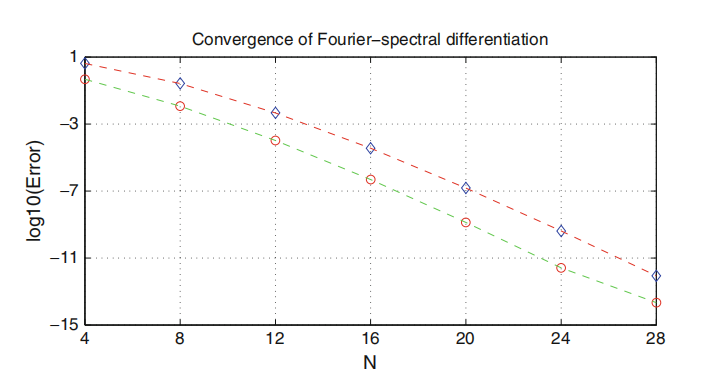
\includegraphics[scale=0.5]{Contents/chapter6/figures/2-1.png}
\caption{一阶($"\circ"$)与二阶($"\diamond"$)傅里叶谱微分的误差}
\label{图2.1}
\end{figure} 
    
    作为数值例子,我们考虑以$2\pi$为周期的函数$u(x) = e^{1 + \sin x}$的傅里叶谱微分。在图\ref{图2.1} 中,我们以半对数标度绘出不同$N$对应的一阶与二阶微分最大逐点误差。图\ref{图2.1}清楚表明了傅里叶谱微分的指数收敛过程。

\subsubsection{球调和方法}

{\color{red}\begin{center}
     邱群
\end{center}}


\subsection{有限元方法}

{\color{red}\begin{center}
     王刘彭
\end{center}}


\subsection{虚单元方法}
{\color{red}\begin{center}
    王鑫
\end{center}}

虚单元方法(VEM)是有限元法(FEM)的推广,它从现代拟有限差分(MFD)格式中得到启发。VEM
允许使用非常一般的多边形和多面体网格,多边形(多面体)网格更容易、更好地剖分区域,
并且自动包含“悬点”.\\

这里以泊松方程为模型来介绍虚单元方法.\\

  \subsubsection{模型:泊松方程}
    
     \begin{equation}\label{eq:dirichlet}
     \begin{cases}
     -\Delta u =f,\qquad  in\quad \Omega.\\
     u=g_D,\qquad on \quad\partial \Omega 
     \end{cases}
     \end{equation}
     $\Omega $是$\mathbb{R}^2$中的多边形区域\\
     
     找到$ u \in H_{g_D}^{1}(\Omega)$:
     \begin{equation}
     (\nabla u,\nabla v)=(f,v) ,\qquad \forall v \in H_0^1(\Omega)
     \end{equation}
     
     其中
     \begin{equation}
     H_{g_D}^{1}=\{u \in H^1(\Omega)\text{且}u|_{ \partial \Omega} = g_D\}\\
     H_{0}^{1}=\{v \in H^1(\Omega)\text{且}u|_{ \partial \Omega} =0\}
     \end{equation}
     
      \subsubsection{二维局部虚单元空间 $\mathcal V_k(E)$}
     \begin{table}[H]
     	\centering
     \begin{tabular}{ cc }   
     	\hline
     	符号 & 含义 \\
     	\hline
     	$E$ & 多边形,可以是非凸的 \\
     	
     	$\Omega$ & 二维有界区域. $\Omega$$\subset$ $\mathbb{R}^2$, $\Omega$ =$\cup_{E\in \mathcal{P}_h}E$ \\
     
     	$V_i$ & $E$ 上逆时针顺序标记的顶点,其中 $i = 1,\cdots, N^V,N^V$ 表示 $E$ 的总的顶点数目 \\
     	
     	$e_i$ & $E$ 中连接 $V_i$ 和 $V_{i+1}$ 的边. 允许两条相邻的边构成 $180$ 度角 \\
     	\hline
     \end{tabular}
     \end{table}
     
    定义函数 $v_h$, $v_h\in\mathcal V_k(E)$ 且满足如下性质:\\
    \\
    $1$) $v_h$ 在 $E$ 的每条边 $e$ 上是一个次数 $\le k$ 多项式, i.e.,$v_h|_e \in \mathcal P_k(e)$\\
    $2$) $v_h$ 在 $E$ 的边界 $\partial E$ 上是全局连续的,i.e.,$v_h|_{\partial E} \in \mathcal C^0(\partial E)$\\
    $3$) $\Delta v_h$ 在 $E$ 内是一个次数 $\le k - 2$ 的多项式, i.e., $\Delta v_h \in \mathcal P_{k-2}(E)$\\
    
    所以 $\mathcal{P}_k(E)$ 是 $V_k(E)$ 子空间. \\
    
    $v_h\in \mathcal V_k(E)$ 的自由度定义如下:\\
    \\
    (1) $v_h$ 在 $E$ 的所有顶点处的函数值\\
    (2) $v_h$ 在 $E$ 的每条除顶点以外的 $k-1$ 个 Gauss-Lobatto 积分点处函数值 \\ 
    (3) $v_h$ 在单元 $E$ 内部与 $\mathcal P_{k-2}(E)$ 中所有单项式 $m_\alpha$ 的乘积的积分平均值, $$ \frac{1}{|E|}\int_E v_h m_\alpha, \quad \alpha = 1, \ldots, n_{k-2}$$
    其中 $n_{k-2} = \dim \mathcal P_{k-2}(E)$\\
    
    易知 $\mathcal V_k(E)$ 的维数为 \\
    \begin{equation}
    N^{dof} = \text{dim} \mathcal V_k(E) = N^V + N^V(k - 1) + n_{k - 2} = N^Vk+ \frac{(k-1)k}{2}.
    \end{equation}
    
    定义从 $V_k(E)$ 到 $\mathbb{R}$ 的算子 $dof_i$ \\
    \begin{equation}
    dof_{i}(v_h) = v_h \text{的第} i \text{个自由度}, \,\ i,j = 1,\cdots, N^{dof} 
    \end{equation}
    
    其中 $N^{dof} := dimV_k(E)$ \\
    
    对于基函数 $\varphi_j \in V_k(E)$ \\
    \begin{equation}
    dof_{i}(\varphi_j) = \delta_{ij},\quad i,j = 1,\cdots,N^{dof} 
    \end{equation}
    
    由于边界自由度在每条边界上都是唯一的次数 $\le k$ 的多项式. 因此, 可以定义全局虚单元空间 $V_h \subset H_0^1(\mathcal D)$ \\
    \begin{equation*}
    V_h := {v_h \in H_0^1(\mathcal D) : \text{对所有} E\in\mathcal{P}_h \text{满足} v_h|_E \in V_k(E)}
    \end{equation*}
    
    $v_h$ 有以下的全局自由度: \\
    \\
    1) $v_h$ 在剖分后的区域的所有内部顶点处的值 \\
    2) $K + 1$ 点 $Guass-Lobatto$ 型求积公式在每条内部边 $e$ 上有 $k - 1$ 个内部积分值, $v_h$ 在所有边内部积分点处的积分值 \\  
    3) 每一个多边形 $E$ 内部的 $n_{k - 2}$个自由度\\
    \begin{equation}
    \frac{1}{|E|}\int_{E}v_hm_{\alpha},\,\ \alpha = 1,\cdots,n_k
    \end{equation}
    
    其中 $n_{k-2} = dim\mathcal{P}_{k - 2}(E)$\\
    
   \subsubsection{计算单元刚度矩阵}
  
    定义在多边形 $E$ 上的 $Laplace$ 算子的单元刚度矩阵\\
    \begin{equation}
    \mathbf(K_E)_{ij} = (\nabla\varphi_i, \nabla\varphi_j)_{0,E},\quad i,j = 1,\cdots,N^{dof}
    \end{equation}
    其中 $\varphi_i \in V_k(E)$ 是 $(2.2)$ 定义的基函数. \\
    
    VEM方法的好处:\\
    
    既不要求使用积分公式也不需要基函数的近似表达式\\
    
     \subsubsection{投影算子 $\Pi^{\nabla}$}
    
    定义 $\Pi^\nabla: \mathcal V_k(E)\rightarrow \mathcal{P}_k(E)$ 如下: 给定  $ v_h \in
    \mathcal V_k(E)$, 找到 $\Pi^\nabla v_h \in \mathcal{P}_k(E)$ 满足: \\
    \begin{equation}
    (\nabla \Pi^\nabla v_h, \nabla p_k) = (\nabla v_h, \nabla p_k), \forall p_k\in\mathcal{P}_k(E)
    \end{equation}
    
    如上所示,满足性质 $(3.2)$ 的 $\Pi^{\nabla}v_h$ 仅为常量,为了确定这个常量可以定义投影: \\
    $ P_0: \mathcal V_k(E) \rightarrow
    \mathcal{P}_0(E)$:
    
    \begin{equation}
    P_0(\Pi^\nabla v_h - v_h) = 0
    \end{equation}
    
    具体定义如下: \\
    \begin{equation}
    \begin{aligned}
    P_0 v_h :=& \frac{1}{N^V}\sum_{i=1}^{N^V} v_h(\mathbf x_i)\text{, for } k=1 \\
    P_0 v_h :=& \frac{1}{|E|} \int_{E}v_h = \frac{1}{|E|} (1, v_h)_E\text{, for } k\geq 2
    \end{aligned}
    \end{equation}
    
    其中 $\frac{1}{|E|} (1, v_h)_E$ 为 $v_h$ 在 $E$ 内部自由度处的值.\\
    
    对于一个给定的 $v_h \in V_k(E)$, 下面展示只使用 $v_h$ 的自由度计算 $\Pi^{\nabla}v_h$ 的过程. \\
    
    因为 $\mathcal M _k(E)$ 是 $\mathcal P_k(E)$ 的一组基,所以让符合性质 $(3.2)$ 的 $p_k$ 只在 $\mathcal M _k(E)$ 范围内变化,即 \\
    \begin{equation}
    (\nabla m_{\alpha}, \nabla(\Pi^{\nabla}v_h) - v_h)_{0,E} = 0,\,\ \alpha = 1,2,\cdots, n_k
    \end{equation}
    
    因为 $\Pi^{\nabla}v_h \in \mathcal P_k(E)$,所以 $\Pi^{\nabla}v_h$ 也可以由基 $\mathcal M_k(E)$ 表示\\
    \begin{equation}
    \Pi^\nabla v_h = \sum_{\beta = 1}s^{\beta}m_\beta
    \end{equation}
    
    把公式 $(3.6)$ 代入公式 $(3.5)$, 得 \\
    \begin{equation}
    \sum_{\beta = 1}^{n_k}s^{\beta}(\nabla m_{\alpha},\nabla m_{\beta})_{0,E} = (\nabla m_{\alpha, \nabla v_h})_{0,E}
    \end{equation}
    
    公式 $(3.7)$ 是由含 $n_k$ 个未知数 $s^{\beta} = s^{\beta}(v_h)$ 的 $n_k$ 个方程组成的线性系统.然而当 $\alpha = 1$ 时, $m_{\alpha} \equiv 1$, 从而方程 $3.7$ 变为 $0 = 0$, 使得方程的解是不确定的. 为了消除这种不确定性,条件 $(3.3)$ 增加一个线性方程: \\
    \begin{equation}
    \sum_{\beta = 1}^{n_k}s^{\beta}P_0m_{\beta} = P_0v_h
    \end{equation}
    那么结合 $(3.7)$ 和 $(3.8)$, 线性方程组可以写成 \\
    \begin{equation*}
    \left[ \begin{array}{cccc}
    P_0m_1 & P_0m_2  &\cdots&P_0m_{n_k} \\
    0 & (\nabla m_2,\nabla m_2)_{0,E} & \cdots & (\nabla m_2,\nabla m_{n_k})_{0,E} \\
    \vdots & \vdots & \ddots & \vdots\\
    0& (\nabla m_{n_k},\nabla m_2)_{0,E} & \cdots & (\nabla m_{n_k},\nabla m_{n_k})_{0,E}
    \end{array} \right]
    \left[ \begin{array}{c}
    s^1\\
    s^2\\
    \vdots\\
    s^{n_k}
    \end{array} \right]
    = \left[\begin{array}{c}
    P_0v_h\\
    (\nabla m_2,\nabla v_h)_{0,E} \\
    \vdots\\
    (\nabla m_{n_k},\nabla v_h)_{0,E} 
    \end{array}\right]
    \end{equation*}
    
    换一种写法,也就是 \\
    \begin{equation}
    G\underline{s} = \underline{b}
    \end{equation}
    
    其中 \\
    \begin{equation}
    G := \begin{bmatrix}
    P_0m_1 & P_0m_1 &\cdots&P_0m_{n_k} \\
    0 & (\nabla m_2,\nabla m_2)_{0,E} & \cdots & (\nabla m_2,\nabla m_{n_k})_{0,E} \\
    \vdots & \vdots & \ddots & \vdots\\
    0& (\nabla m_{n_k},\nabla m_2)_{0,E} & \cdots & (\nabla m_{n_k},\nabla m_{n_k})_{0,E}
    \end{bmatrix}\\
    \end{equation}
    \begin{equation}
    \underline b := \begin{bmatrix}
    P_0v_h\\
    (\nabla m_2,\nabla v_h)_{0,E} \\
    \vdots\\
    (\nabla m_{n_k},\nabla v_h)_{0,E} 
    \end{bmatrix}
    \end{equation}
    
    假定 $E$ 上的多项式的积分是可以计算的, 公式 $(3.10)$ 中的矩阵 $G$ 是可以计算的. \\
    \subsubsection{计算 $\Pi^{\nabla}$}

对每个基函数$\varphi_i$,定义$s_i^{\alpha}$为$\Pi^{\nabla}\varphi_i$由基$m_{\alpha}$表示的系数: \\
\begin{equation}
\Pi^\nabla \varphi_i = \sum_{\alpha = 1}^{n_k}s_{i}^{\alpha}m_\alpha,\quad i = 1,\cdots,N^{dof}
\end{equation}

在公式 $(3.9)$ 的右端项中用$\varphi_i$代替$v_h$,$s_i^{\alpha}$是下列方程的解: \\
\begin{equation*}
 \left[\begin{array}{cccc}
P_0m_1 & P_0m_1 &\cdots&P_0m_{n_k} \\
0 & (\nabla m_2,\nabla m_2)_{0,E} & \cdots & (\nabla m_2,\nabla m_{n_k})_{0,E} \\
\vdots & \vdots & \ddots & \vdots\\
0& (\nabla m_{n_k},\nabla m_2)_{0,E} & \cdots & (\nabla m_{n_k},\nabla m_{n_k})_{0,E}
\end{array}\right]
\left[\begin{array}{c}
s_i^1\\
s_i^2\\
\vdots\\
s_i^{n_k}
\end{array}\right]
= \left[\begin{array}{c}
P_0\varphi_i\\
(\nabla m_2,\nabla \varphi_i)_{0,E} \\
\vdots\\
(\nabla m_{n_k},\nabla \varphi_i)_{0,E}
\end{array}\right]
\end{equation*}

换一种形式为: \\
\begin{equation*}
\underline s^{(i)} = G^{-1}\underline b^{(i)}
\end{equation*}

把 $n_k \times N^{dof}$ 矩阵 $B$ 记为 \\
\begin{equation}
\begin{aligned}
B &:= \begin{bmatrix}
b^{(1)} & b^{(2)} & \cdots & b^{(N^{dof})}
\end{bmatrix} \\
& = \begin{bmatrix}
P_0\varphi_1 & \cdots & P_0\varphi_{N^{dof}}\\
(\nabla m_2, \nabla\varphi_1)_{0, E} & \cdots & (\nabla m_2, \nabla\varphi_{N^{dof}})_{0, E}\\
\cdots & \cdots & \cdots \\
(\nabla m_{n_k}, \nabla\varphi_1)_{0, E} & \cdots & (\nabla m_{n_k}, \nabla\varphi_{N^{dof}})_{0, E}\\
\end{bmatrix}\\
& = \begin{bmatrix}
P_0\varphi_1 & \cdots & P_0\varphi_{N^{dof}}\\
-(\Delta m_2,\varphi_1)_{0, E} & \cdots & -(\Delta m_2,\varphi_{N^{dof}})_{0, E}\\
\cdots & \cdots & \cdots \\
-(\Delta m_{n_k}, \varphi_1)_{0, E} & \cdots & -(\Delta m_{n_k},\varphi_{N^{dof}})_{0, E}\\
\end{bmatrix}\\
& +\begin{bmatrix}
0 & \cdots & 0\\
(\frac{ \partial m_2}{\partial \mathbf n},\varphi_1)_{\partial E} & \cdots & (\frac{\partial m_2}{\partial \mathbf n},\varphi_{N^{dof}})_{\partial E}\\
\cdots & \cdots & \cdots \\
(\frac{\partial m_{n_k}}{\partial \mathbf n}, \varphi_1)_{\partial E} & \cdots & (\frac{\partial m_{n_k}}{\partial \mathbf n}, \varphi_{N^{dof}})_{\partial E}\\
\end{bmatrix}\\
\end{aligned}
\end{equation}

算子 $\Pi^{\nabla}$ 的矩阵表达 $\boldsymbol{\Pi}_{\ast}^{\nabla}$: 由$V_k{E}$ 到 $\mathcal{P}_k(E)$ 的基 $\mathcal{M}_k(E)$ 的映射,通过 \\
\begin{equation*}
(\boldsymbol{\Pi}_{\ast}^{\nabla})_{\alpha i} = s_i^{\alpha}
\end{equation*}

给出,也就是 \\
\begin{equation}
\boldsymbol{\Pi}_{\ast}^{\nabla} = G^{-1}B
\end{equation}

令 \\
\begin{equation*}
\Pi^{\nabla} \varphi_i = \sum_{j=1}^{N^{dof}}\pi_i^j \varphi_j, \quad i = 1,\cdots,N^{dof}
\end{equation*}

其中 \\
\begin{equation*}
\pi_i^j = dof_j(\Pi^{\nabla}\varphi_i)
\end{equation*}

从公式 $(3.13)$ 和 $(2.3)$,可得 \\
\begin{equation*}
\Pi^{\nabla} \varphi_i = \sum_{\alpha=1}^{n_k}s_i^{\alpha}\sum_{j=1}^{N^{dof}}dof_j(m_{\alpha})\varphi_j
\end{equation*}

因此 \\
\begin{equation}
\pi_i^j = \sum_{\alpha=1}^{n_k}s_i^{\alpha}dof_j(m_{\alpha})
\end{equation}

为了用矩阵表示公式 $(3.16)$, 定义 $N^{dof}\times n_k$ 维矩阵 $D$ \\
\begin{equation*}
D_{i\alpha} := dof_i(m_{\alpha})\quad i = 1,\cdots,N^{dof},\quad\alpha = 1,\cdots,n_k
\end{equation*}

即 \\
\begin{equation}
D = \begin{bmatrix}
dof_1(m_1) & dof_1(m_2) & \cdots & dof_1(m_{n_k})\\
dof_2(m_1) & dof_2(m_2) & \cdots & dof_2(m_{n_k})\\
\vdots & \vdots & \ddots & \vdots\\
dof_{N^{dof}}(m_1) & dof_{N^{dof}}(m_2) & \cdots & dof_{N^{dof}}(m_{n_k})\\
\end{bmatrix}
\end{equation}

方程 $(3.16)$ 变为 \\
\begin{equation*}
\pi_i^j = \sum_{\alpha=1}^{n_k}(G^{-1}B)_{\alpha i}D_{j \alpha} = \sum_{\alpha=1}^{n_k}D_{j \alpha}(G^{-1}B)_{\alpha i} = (DG^{-1}B)_{ji}
\end{equation*}

因此,算子 $\Pi^{\nabla}:V_k(E) \to V_k(E)$在基 $(2.2)$ 的矩阵表达 $\boldsymbol{\Pi}^{\nabla}$ 满足 \\
\begin{equation}
\boldsymbol{\Pi}^{\nabla} = D G^{-1} B = D \boldsymbol{\Pi}_{\ast}^{\nabla}
\end{equation}

注解 \\
\begin{equation}
G = BD
\end{equation}
证明如下: \\

当 $\alpha = 1$ 时
\begin{equation*}
\begin{aligned}
\sum_{i = 1}^{N^{dof}}{B}_{1i}{D}_{i\beta} & = \sum_{i = 1}^{N^{dof}}P_0\varphi_idof_i(m_{\beta}) \\
& = P_0(\sum_{i = 1}^{N^{dof}}\varphi_idof_i(m_{\beta})) \\& = P_0m_{\beta} \\
& = G_{1\beta}
\end{aligned}
\end{equation*}

当 $\alpha \ge 2$ 时 \\
\begin{equation*}
\begin{aligned}
\sum_{i = 1}^{N^{dof}}{B}_{\alpha i}{D}_{i\beta} & = \sum_{i = 1}^{N^{dof}}(\nabla m_{\alpha},\nabla \varphi_i)_{0,E}dof_i(m_{\beta}) \\
& = (\nabla m_{\alpha},\sum_{i = 1}^{N^{dof}}dof_i(m_{\beta})\nabla \varphi_i)_{0,E} \\
& = (\nabla m_{\alpha},\nabla(\sum_{i = 1}^{N^{dof}}dof_i(m_{\beta})\varphi_i))_{0,E} \\
& = (\nabla m_{\alpha},\nabla m_{\beta})_{0,E} \\
& = G_{\alpha\beta}
\end{aligned}
\end{equation*}

我们使用公式 $(3.10)$ 计算 $G$, 使用公式 $(3.19)$ 检验 $B, D, G$ 的正确性.\\
\subsubsection{单元刚度矩阵构造}

定义在多边形 $E$ 上的 Laplace 算子的单元刚度矩阵. 利用投影算子$\Pi^{\nabla}$, 作分解: \\
\begin{equation*} 
\varphi_i = \Pi^{\nabla} \varphi_i + (I-\Pi^{\nabla})\varphi_i 
\end{equation*}

\begin{equation*} 
\varphi_j = \Pi^{\nabla} \varphi_j + (I-\Pi^{\nabla})\varphi_j
\end{equation*}

把上式代入到 $(3.1)$, 然后展开可得 \\
\begin{equation*}
\begin{aligned}
(\mathbf K_{E})_{i j} = & (\nabla(\Pi^{\nabla} \varphi_i + (I-\Pi^{\nabla})\varphi_i),\nabla(\Pi^{\nabla} \varphi_j + (I-\Pi^{\nabla})\varphi_j)) \\
=& (\nabla \Pi^{\nabla} \varphi_i, \nabla \Pi^{\nabla} \varphi_j) + (\nabla(I-\Pi^{\nabla})\varphi_i,\nabla(I-\Pi^{\nabla})\varphi_j)\\
& + (\nabla \Pi^{\nabla} \varphi_i,\nabla(I-\Pi^{\nabla})\varphi_j)+(\nabla(I-\Pi^{\nabla})\varphi_i,\nabla \Pi^{\nabla} \varphi_j)\\ 
= &(\nabla \Pi^{\nabla} \varphi_i, \nabla \Pi^{\nabla} \varphi_j) + (\nabla(I-\Pi^{\nabla})\varphi_i,\nabla(I-\Pi^{\nabla})\varphi_j)
\end{aligned}
\end{equation*}

第二个等号到第三个等号: \\

由投影算子 $\Pi^{\nabla}$ 的定义可知,后两项为 $0$,所以等号是成立的.\\

单元刚度矩阵的第 $1$ 项确保一致性,可以精确计算; 第 $2$ 项确保稳定性,可以近似求解.从文献 $5$ 中可知\\

我们选择标准基函数 $\varphi_1,\cdots,\varphi_{N^{dof}}$: \\
\begin{equation}
\chi_i(\varphi_j) = \delta_{ij},\quad i,j = 1,2,\cdots,N^{dof}
\end{equation}

A0.3: 假设 $\exists \gamma > 0$ s.t. 对 $\forall h$ 和每个单元 $E \in \mathcal{P}_h$ 并且在 $E$ 的任意两个顶点之间的距离都 $\ge \gamma h_E$.

在 A0.3 的前提下,有 \\
\begin{equation*}
(\nabla(I-\Pi^{\nabla})\varphi_i,\nabla(I-\Pi^{\nabla})\varphi_j) = \sum_{r = 1}^{N^{dof}} \chi_r((I-\Pi^{\nabla})\varphi_i) \chi_r((I-\Pi^{\nabla})\varphi_j)
\end{equation*}

由 $(3.20)$ 和 $(2.2)$ 可知 \\
\begin{equation}
\begin{aligned}
(\nabla(I-\Pi^{\nabla})\varphi_i,\nabla(I-\Pi^{\nabla})\varphi_j) & = \sum_{r = 1}^{N^{dof}} \chi_r((I-\Pi^{\nabla})\varphi_i) \chi_r((I-\Pi^{\nabla})\varphi_j) \\
& = \sum_{r = 1}^{N^{dof}} dof_r((I-\Pi^{\nabla})\varphi_i) dof_r((I-\Pi^{\nabla})\varphi_j) \\
\end{aligned}
\end{equation}

现在单元刚度矩阵可以写为 \\
\begin{equation}
(K_{E}^h)_{ij} := (\nabla \Pi^{\nabla}\varphi_i, \nabla \Pi^{\nabla}\varphi_j)_{0,E} + \sum_{r = 1}^{N^{dof}} dof_r((I-\Pi^{\nabla})\varphi_i) dof_r((I-\Pi^{\nabla})\varphi_j)
\end{equation}

这样就把虚单元法单元刚度矩阵的计算分解为可计算的两部分, 其中第一部分从公式
$(3.13)$ 可知 \\
\begin{equation}
\begin{aligned}
&\begin{bmatrix}
(\nabla\Pi^\nabla\varphi_1, \nabla\Pi^\nabla\varphi_1) & (\nabla\Pi^\nabla\varphi_1, \nabla\Pi^\nabla\varphi_2) & \cdots & (\nabla\Pi^\nabla\varphi_1, \nabla\Pi^\nabla\varphi_{N^{dof}})\\
(\nabla\Pi^\nabla\varphi_2, \nabla\Pi^\nabla\varphi_1) & (\nabla\Pi^\nabla\varphi_2, \nabla\Pi^\nabla\varphi_2) & \cdots & (\nabla\Pi^\nabla\varphi_2, \nabla\Pi^\nabla\varphi_{N^{dof}})\\
\cdots & \cdots & \cdots & \cdots \\
(\nabla\Pi^\nabla\varphi_{N^{dof}}, \nabla\Pi^\nabla\varphi_1) & (\nabla\Pi^\nabla\varphi_{N^{dof}}, \nabla\Pi^\nabla\varphi_2) & \cdots & (\nabla\Pi^\nabla\varphi_{N^{dof}}, \nabla\Pi^\nabla\varphi_{N^{dof}})\\
\end{bmatrix}\\
& = \int_E \begin{bmatrix} 
\nabla\Pi^\nabla\varphi_1\\ 
\nabla\Pi^\nabla\varphi_2 \\ 
\vdots\\
\nabla\Pi^\nabla\varphi_{N^{dof}}
\end{bmatrix}\begin{bmatrix} 
\nabla\Pi^\nabla\varphi_1\\ 
\nabla\Pi^\nabla\varphi_2 \\ 
\vdots\\
\nabla\Pi^\nabla\varphi_{N^{dof}}
\end{bmatrix}^T\mathrm d \mathbf x\\
& = \int_E \begin{bmatrix} 
\nabla(\sum_{\alpha = 1}^{n_k}(\Pi_{*}^{\nabla})_{\alpha 1}\cdot m_{\alpha})\\ 
\nabla(\sum_{\alpha = 1}^{n_k}(\Pi_{*}^{\nabla})_{\alpha 2}\cdot m_{\alpha}) \\ 
\vdots\\
\nabla(\sum_{\alpha = 1}^{n_k}(\Pi_{*}^{\nabla})_{\alpha N^{dof}}\cdot m_{\alpha})
\end{bmatrix}\begin{bmatrix} 
\nabla(\sum_{\alpha = 1}^{n_k}(\Pi_{*}^{\nabla})_{\alpha 1}\cdot m_{\alpha})\\ 
\nabla(\sum_{\alpha = 1}^{n_k}(\Pi_{*}^{\nabla})_{\alpha 2}\cdot m_{\alpha}) \\ 
\vdots\\
\nabla(\sum_{\alpha = 1}^{n_k}(\Pi_{*}^{\nabla})_{\alpha N^{dof}}\cdot m_{\alpha})
\end{bmatrix}^T\mathrm d \mathbf x\\
\end{aligned}
\end{equation}
\begin{equation*}
    \begin{aligned}
& = \int_E \begin{bmatrix} 
(\sum_{\alpha = 1}^{n_k}(\Pi_{*}^{\nabla})_{\alpha 1}\cdot \nabla m_{\alpha})\\ 
(\sum_{\alpha = 1}^{n_k}(\Pi_{*}^{\nabla})_{\alpha 2}\cdot \nabla m_{\alpha}) \\ 
\vdots\\
(\sum_{\alpha = 1}^{n_k}(\Pi_{*}^{\nabla})_{\alpha N^{dof}}\cdot \nabla m_{\alpha})
\end{bmatrix}\begin{bmatrix} \\
(\sum_{\alpha = 1}^{n_k}(\Pi_{*}^{\nabla})_{\alpha 1}\cdot \nabla m_{\alpha})\\ 
(\sum_{\alpha = 1}^{n_k}(\Pi_{*}^{\nabla})_{\alpha 2}\cdot \nabla m_{\alpha}) \\ 
\vdots\\
(\sum_{\alpha = 1}^{n_k}(\Pi_{*}^{\nabla})_{\alpha N^{dof}}\cdot \nabla m_{\alpha})
\end{bmatrix}^T \mathrm d \mathbf x \\
& = \int_{E} \begin{bmatrix} 
(\Pi_{*}^{\nabla})_{1 1} & (\Pi_{*}^{\nabla})_{2 1} & \cdots  & (\Pi_{*}^{\nabla})_{n_k 1} \\ 
((\Pi_{*}^{\nabla})_{1 2} & (\Pi_{*}^{\nabla})_{2 2} & \cdots  & (\Pi_{*}^{\nabla})_{n_k 2} \\ 
\vdots\\
(\Pi_{*}^{\nabla})_{1 N^{dof}} & (\Pi_{*}^{\nabla})_{2 N^{dof}} & \cdots  & (\Pi_{*}^{\nabla})_{n_k N^{dof}}
\end{bmatrix}
\begin{bmatrix} 
\nabla m_{1}\\ 
\nabla m_{2} \\ 
\vdots\\
\nabla m_{n_k}
\end{bmatrix}  \\
&\begin{bmatrix} 
\nabla m_{1} & \nabla m_{2} & \cdots &\nabla m_{n_k}
\end{bmatrix}
\begin{bmatrix} 
(\Pi_{*}^{\nabla})_{1 1} & (\Pi_{*}^{\nabla})_{1 2} & \cdots  & (\Pi_{*}^{\nabla})_{1 N^{dof}} \\ 
((\Pi_{*}^{\nabla})_{2 1} & (\Pi_{*}^{\nabla})_{2 2} & \cdots  & (\Pi_{*}^{\nabla})_{2 N^{dof}} \\ 
\vdots\\
(\Pi_{*}^{\nabla})_{n_k 1} & (\Pi_{*}^{\nabla})_{n_k 2} & \cdots  & (\Pi_{*}^{\nabla})_{n_k N^{dof}}
\end{bmatrix} \mathrm d \mathbf x\\
= & \int_E [\boldsymbol \Pi_{*}^\nabla]^T \begin{bmatrix}
\nabla m_1 \\ \nabla m_2 \\\vdots\\ \nabla m_{n_k}
\end{bmatrix}
(\nabla m_1, \nabla m_2, \cdots,  \nabla m_{n_k}) \boldsymbol \Pi_{*}^{\nabla} \mathrm d \mathbf x \\
= & [\boldsymbol \Pi_{*}^\nabla]^T \tilde{G} \boldsymbol \Pi_{*}^\nabla
\end{aligned}
\end{equation*}

其中 $\tilde{G}$ 的第一行元素都为 0,其它元素与 $G$ 保持一致.\\

第二项的计算如下: \\
\begin{equation}
\begin{aligned}
\sum_{r = 1}^{N^{dof}} \chi_r((I-\Pi^{\nabla})\varphi_i) \chi_r((I-\Pi^{\nabla})\varphi_j) & = \sum_{r = 1}^{N^{dof}} (\mathbf{I} - \boldsymbol {\Pi^{\nabla}})_{ri}\boldsymbol {\Pi^{\nabla}})_{ri} \\
& = \sum_{r = 1}^{N^{dof}} (\mathbf{I} - \boldsymbol {\Pi^{\nabla}})_{ir}^T\boldsymbol {\Pi^{\nabla}})_{ri} \\
& = \begin{bmatrix}(\mathbf{I} - \boldsymbol {\Pi^{\nabla}})^T(\mathbf{I} - \boldsymbol {\Pi^{\nabla}})\end{bmatrix}_{ij}
\end{aligned}
\end{equation}

最后可以得到单元刚度矩阵的矩阵表达式: \\
\begin{equation}
\mathbf K_E^h = [\boldsymbol \Pi^\nabla_{*}]^T \tilde{G} \boldsymbol \Pi_{*}^\nabla + (\mathbf I - \boldsymbol \Pi^\nabla)^T(\mathbf I - \boldsymbol \Pi^\nabla)
\end{equation}


\subsubsection{$k = 1$ 时的情况}

当 $k=1$ 时,容易给出$\Pi^{\nabla} v_h$的公式。因为1次多项式的梯度为常向量,方程 $(3.2)$ 可化为 \\
\begin{equation}
|E| \nabla p_1 \cdot \nabla(\Pi^{\nabla}v_h) = \nabla p_1 \cdot \int_E \nabla v_h
\end{equation}

过程: \\
\begin{equation*}
\begin{aligned}
(\nabla p_1, \nabla(\Pi^\nabla v_h - v_h))_{0,E} & = 0 \\
\Rightarrow
(\nabla p_1, \nabla\Pi^\nabla v_h)_{0,E} & = (\nabla p_1, \nabla v_h)_{0,E} \\
\Rightarrow
|E| \nabla p_1 \cdot \nabla(\Pi^{\nabla}v_h) & = \nabla p_1 \cdot \int_E \nabla v_h
\end{aligned}
\end{equation*}

通过取$p_1 = x_1,p_1 =x_2$,方程 $(3.26)$ 等价于 \\
\begin{equation}
\mathbf g(v_h) := \nabla(\Pi^{\nabla} v_h) = \frac{1}{|E|} \int_E \nabla v_h
\end{equation}

因此 \\
\begin{equation}
\Pi^{\nabla} v_h = x\mathbf g(v_h) + c
\end{equation}

这里,$c$是取决于$v_h$的常量函数。\\

有了表达式 $(3.28)$,我们可以计算出公式 $(3.22)$ 中的一致项。\\

由定义 $(3.27)$,方程 $(3,23)$ 右端第一项变为 \\
\begin{equation*}
(\nabla\Pi^{\nabla} \varphi_i,\nabla\Pi^{\nabla} \varphi_j)_{0,E}=|E|\mathbf g(\varphi_i)\mathbf g(\varphi_j)
\end{equation*}

因为 $\varphi_i$ 在每条边上都是线性的,容易知道 \\
\begin{equation}
|E|\mathbf g(\varphi_i) \equiv \int_E \nabla \varphi_i = \frac{1}{2} (|e_{i-1}| \mathbf{n}_{i-1} + |e_i| \mathbf{n}_i) = \frac{1}{2} \mathbf{d}_i^\perp
\end{equation}

其中,符号 $\perp$ 表示逆时针旋转 $90^\circ$, \\
\begin{equation*}
\mathbf{d}_i = V_{i-1}-V_{i+1}
\end{equation*}

\begin{equation*}
\mathbf{d}_i^{\perp}=\begin{bmatrix}0&-1\\1&1\end{bmatrix}\mathbf{d}_i
\end{equation*}

下面证明 $\int_E \nabla \varphi_i = \frac{1}{2} (|e_{i-1}| \mathbf{n}_{i-1} + |e_i| \mathbf{n}_i)$:

证明:记 $V = (x,y)^T$ 为多边形边界上任意一点,$V_i$ 为多边形顶点,$e_i$ 为 $V_iV_{i+1}$, $\mathbf{n}_i$ 为边 $e_i$ 上的单位外法向量. \\

令 $V = (1 - t)V_i + tV_{i + 1}$, 则 \\
\begin{equation*}
\begin{aligned}
x(t) & = (1 - t)x_i + tx_{i + 1} \\
y(t) & = (1 - t)y_i + ty_{i + 1} \\
x'(t) & = x_{i + 1} - x_i \\
y'(t) & = y_{i + 1} - y_i
\end{aligned}
\end{equation*}

记 $\tilde{\varphi}_i = \varphi_i(V)$, 由于 $\varphi$ 在边界上为线性多项式,且 \\
\begin{equation*}
\varphi_i(V_i) = 1,\,\ \varphi_i(V_j) = 0\,\ (i\ne j)
\end{equation*}

则可设 \\
\begin{equation*}
\begin{aligned}
\tilde{\varphi}_i(t) & = at + b \\
\tilde{\varphi}_i(0) & = \varphi_i(V_i),\,\ \text{即} b = 1 \\
\tilde{\varphi}_i(1) & = \varphi_i(V_{i+1}),\,\ \text{即} a + b = 0 \\
\text{则} \,\ \tilde{\varphi}_i(t) & = 1 - t 
\end{aligned}
\end{equation*}

从而 \\
\begin{equation*}
\begin{aligned}
\int_{e_i}\varphi_i & = \int_0^1 \tilde{\varphi}_i(t)\sqrt{\begin{bmatrix}x'(t)\end{bmatrix}^2 + \begin{bmatrix}y'(t)\end{bmatrix}^2} \mathrm dt\\ 
& = \int_0^1 \tilde{\varphi}_i(t)\sqrt{(x_{i+1} - x_i)^2 + (y_{i+1} - y_i)^2} \mathrm dt \\
& = |e_i|\int_0^1\tilde \varphi_i(t) \mathrm dt \\
& = |e_i|\int_0^1(1 - t) \mathrm dt \\
& = \frac{1}{2}|e_i|
\end{aligned}
\end{equation*}

类似可得 \\
\begin{equation*}
\int_{e_{i - 1}}\varphi_i = \frac{1}{2}|e_{i - 1}|
\end{equation*}

从而 \\
\begin{equation*}
\begin{aligned}
|E|g(\varphi_i) & = \int_{E} \nabla \varphi_i \\
& = \begin{pmatrix}
\int_{E} \frac{\partial \varphi_i}{\partial x} \\
\\
\int_{E} \frac{\partial \varphi_i}{\partial y}
\end{pmatrix} \\
& = \begin{pmatrix}
\int_{E} div\begin{pmatrix}
\varphi_i \\
0
\end{pmatrix} \\
\\
\int_{E} div\begin{pmatrix}
0 \\
\varphi_i 
\end{pmatrix} 
\end{pmatrix} \\
& = \begin{pmatrix}
\int_{\partial E} \begin{pmatrix}
\varphi_i \\
0
\end{pmatrix}\cdot \mathbf n \\
\\
\int_{\partial E} \begin{pmatrix}
0 \\
\varphi_i 
\end{pmatrix}\cdot \mathbf n \\
\end{pmatrix} \\
& = \begin{pmatrix}
\int_{\partial E} \varphi_i n_x \\
\\
\int_{\partial E} \varphi_i n_x 
\end{pmatrix} \\
& = \int_{\partial E} \varphi_i \mathbf n \\
& = \int_{e_{i - 1}}\varphi_i \mathbf {n}_{i - 1} + \int_{e_{i}}\varphi_i \mathbf {n}_{i} \\
& = \frac{1}{2}(|e_{i - 1}|\mathbf{n}_{i - 1} + |e_i|\mathbf{n}_i)
\end{aligned}
\end{equation*}
其中 $\mathbf{n}$ 为 $\partial E$ 上的单位外法向量. \\

因此 \\
\begin{equation*}
(\nabla\Pi^{\nabla} \varphi_i,\nabla\Pi^{\nabla} \varphi_j)_{0,E} = \frac{1}{4|E|} \mathbf{d}_i^\perp \cdot \mathbf{d}_j^\perp = \frac{1}{4|E|} \mathbf{d}_i \cdot \mathbf{d}_j
\end{equation*}

为了获得公式 $(3.22)$ 中的稳定项,需要计算$\Pi^{\nabla}\varphi_i$的自由度,在 $k=1$ 时只需 $\Pi^{\nabla}\varphi_i$ 在多边形 $E$ 顶点处的值。首先,需要知道 $(3.28)$ 中的常量$c$。从 $(3.3)$ 可得 \\
\begin{equation}
P_0(\Pi^{\nabla}v_h) \equiv P_0(x) \cdot \mathbf g(v_h) + P_0c = P_0 v_h
\end{equation}

明显有 $P_0c=c$,回顾方程 $(3.4)$,定义$\bar{V}, \bar{v}_h$为结点中心的坐标和$v_h$的平均结点值。\\
\begin{equation*}
\begin{aligned}
\bar{V} &:= P_0(x) = \frac{1}{N^V} \sum_{i=1}^{N^V}V_i\\
\bar{v}_h &:= P_0v_h = \frac{1}{N^V}\sum_{i=1}^{N^V}v_h(V_i)
\end{aligned}
\end{equation*}

从 $(3.30)$ 可以推出 \\
\begin{equation*}
c= P_0 v_h - P_0(x) \cdot \mathbf g(v_h) =\bar{v}_h - \bar{V}\cdot \mathbf g(v_h)
\end{equation*}

因此 \\
\begin{equation*}
\Pi^{\nabla}v_h = (x-\bar{V}) \cdot g(v_h) + \bar{v}_h
\end{equation*}

用$\varphi_i$代替$v_h$,代入上式,在利用 $(3.29)$,可以得到 \\
\begin{equation*}
\Pi^{\nabla}\varphi_i = \frac{1}{2|E|} (x-\bar{V})\cdot \mathbf{d}_i^\perp + \frac{1}{N^V} 
\end{equation*}

因此 \\
\begin{equation}
(\Pi^{\nabla})_{ri} = dof_r(\Pi^{\nabla} \varphi_i) = (\Pi^{\nabla} \varphi_i)(V_r) =  \frac{1}{2|E|} (V_r-\bar{V})\cdot\mathbf{d}_i^\perp + \frac{1}{N^V}
\end{equation}

导出 \\
\begin{equation}
(I-\Pi^{\nabla})_{ri} = dof_r(I-\Pi^{\nabla} \varphi_i) = (\delta_{ir} - \frac{1}{N^V})- \frac{1}{2|E|} (V_r-\bar{V})\cdot \mathbf{d}_i^\perp 
\end{equation}

\subsubsection{$L^2$ 投影}

我们给出 $v_h \in V_k(E)$ 的自由度. 参考前面的部分我们可以得到 $v_h$ 的信息: \\
\begin{flalign}
\begin{split}
& 1). v_h\text{在多边形} E \text{的边上的} \text{的每点的值}; \\
& 2). v_h\text{在次数} \le k - 2 \text{的多项式空间上的} L^2 \text{投影}; \\
& 3). v_h \text{在次数} \le k \text{的多项式空间的投影}\Pi^{\nabla}v_h. \\
\end{split}
\end{flalign}

这样我们可以通过计算右端项 $(\mathbf{b}_E)_i = \int_Ef\varphi_i$ 得到 $\mathbf{b}_E^h$ 的近似. \\

这个近似确保 $VEM$ 的解 $u_h$ 满足最佳误差估计: \\
\begin{equation*}
||u - u_h||_{0,\Omega} = O(h^{k+1}),\quad ||\nabla u - \nabla u_h||_{0,\Omega} = O(h^{k})
\end{equation*}

\subsubsection{$L^2$ 投影的定义与性质}

对于每个 $v_h \in V_h$, 定义投影算子 $\Pi^0:\mathcal V_k(E)\to \mathcal P_k(E)$, 满足: \\
\begin{equation}
(p_k, \Pi^0 v_h - v_h)_{0,E} = 0, \quad \forall p_k \in \mathcal P_k(E)
\end{equation}

与第三部分类似,我们定义矩阵 \\
\begin{equation}
H_{\alpha \beta} := (m_\alpha, m_\beta)_{0,E}\quad \alpha,\beta = 1,2,\cdots, n_k
\end{equation}

$t^{\alpha} = t^{\alpha}(v_h)$ 是 $\Pi^0v_h$ 在基 $m_\alpha$ 处的系数: \\

\begin{equation}
\Pi^0v_h = \sum_{\alpha = 1}^{n_k}t^{\alpha}m_{\alpha}
\end{equation}

因为$\mathcal{M}_k(E)$是$\mathcal{P}_k(E)$的一组基,让符合性质 $(4.2)$ 的$p_k$只在$\mathcal{M}_k(E)$范围内变化,即 \\
\begin{equation*}
(m_{\alpha}, \Pi^0 v_h)_{0,E} = (m_{\alpha}, v_h)_{0,E}, \quad \forall m_{\alpha} \in \mathcal {P}_k(E)\,\ \alpha =1,...,n_k
\end{equation*}

把 $(4.4)$ 代入上式中可以得到 \\
\begin{equation*}
\sum_{\beta = 1}^{n_k}t^{\beta}(m_{\alpha}, m_{\beta})_{0,E} = (m_{\alpha}, v_h)_{0,E}\quad \alpha =1,...,n_k 
\end{equation*}

令 \\
\begin{equation}
c^{\alpha}:= (m_{\alpha},v_h)_{0,E}
\end{equation}

即 \\
\begin{equation*}
\begin{bmatrix}
(m_1,m_1)_{0,E} & (m_1,m_2)_{0,E} & \cdots & (m_1,m_{n_k})_{0,E} \\
(m_2,m_1)_{0,E} & (m_2,m_2)_{0,E} & \cdots &
(m_2,m_{n_k})_{0,E} \\
\vdots & \vdots & \ddots & \vdots \\
(m_{n_k}, m_1)_{0,E} & (m_{n_k},m_2)_{0,E} & \cdots & (m_{n_k},m_{n_k})_{0,E}
\end{bmatrix}\begin{bmatrix}
t^1 \\
t^2 \\
\vdots \\
t^{n_k}
\end{bmatrix}
= \begin{bmatrix}
(m_1,v_h)_{0,E} \\
(m_2,v_h)_{0,E} \\
\vdots \\
(m_{n_k},v_h)_{0,E}
\end{bmatrix} 
\end{equation*}

我们也可以简记为 \\
\begin{equation}
\mathbf{H}\underline{t} = \underline{c}\quad \text{that is} \quad \underline{t} = \mathbf{H}^{-1}\underline{c}
\end{equation}

我们仅仅使用 $v_h$ 的自由度计算 $(4.5)$ 中 $\underline{c}$.\\

我们知道,对于每一个 $v_h \in \mathcal{V}_k(E)$,计算 $\Pi^{\nabla}v_h$ 的时候仅仅使用 $v_h$ 的自由度.\\

那么我们指出,对于每一个 $v_h \in \mathcal{V}_k(E)$, $\Pi^{\nabla}v_h$ 和 $\Pi^{0}v_h$ 都是 $v_h$ 很好的近似,并且当 $v_h$ 在多项式空间 $\mathcal{P}_{k}(E)$ 时与 $v_h$ 一致.因此,它们非常相近.\\

那么对于次数为 $k$ 和 $k_1$ 的单项式 $m_{\alpha}$, 我们可以使用下式代替 $(4.5)$: \\
\begin{equation}
c^{\alpha}:= (m_{\alpha},\Pi^{\nabla}v_h)_{0,E}
\end{equation}

通过 $v_h$ 的自由度计算.\\

我们引入一个新的空间 $W_k(E)$, 且它满足 $\mathcal{V}_k(E)$ 的全部的好的性质: \\

* 在 E 的每条边 e 上 $W_K(E)$ 的元素都是 k 次多项式;  \\

* $\mathcal {P}_k(E)\subset W_k(E)$;  \\

* 在 $W_k(E)$ 中我们使用与 $\mathcal{V}_k(E)$ 相同的自由度. \\ 

再加一个性质  \\
\begin{equation}
\int_{E} w_hm_{\alpha} = \int_{E}\Pi^{\nabla} w_h m_{\alpha}\quad |\alpha| = k-1,k,\,\ w_h \in W_k(E)
\end{equation}

此时,$(4.5)$ 和 $(4.7)$ 是等价的.\\

\subsubsection{ $k = 1, k = 2$ 的例子}

如果 $k = 1 \quad\text{or}\quad k = 2$, 我们容易得到 $\Pi^\nabla = \Pi^0$. \\

1). $k = 1$ \\

由方程 $(4.2)$ 可知 \\
\begin{equation*}
(p_1,\Pi^0 v_h)_{0,E} = (p_1,v_h)_{0,E},\quad p_1 \in \mathcal{P}_1(E)
\end{equation*}

公式 $(4.8)$ 中的 $w_h$ 换成 $v_h$, $m_\alpha$ 换成 $p_1$, 有 \\
\begin{equation*}
(p_1,\Pi^\nabla v_h)_{0,E} = (p_1,v_h)_{0,E},\quad p_1 \in \mathcal{P}_1(E)
\end{equation*}

因此 \\
\begin{equation*}
\Pi^\nabla = \Pi^0
\end{equation*}

2). $k = 2$: \\

由条件 $(3.3)$ 和定义 $(3.4)$, 有 \\
\begin{equation*}
(1,\Pi^\nabla v_h)_{0,E} = (1,v_h)_{0,E}
\end{equation*}

证明如下: \\
\begin{equation*}
\begin{aligned}
P_0(\Pi^\nabla v_h - v_h) & = 0 \\
\Rightarrow \Pi^\nabla v_h - P^0 v_h & = 0 \\
\Rightarrow \Pi^\nabla v_h & = \frac{1}{|E|} \int_{E}v_h \\
\Rightarrow |E|\Pi^\nabla v_h & = \int_{E}v_h \\
\Rightarrow \int_{E}\Pi^\nabla v_h & = \int_{E}v_h \\
\Rightarrow (1,\Pi^\nabla v_h)_{0,E} & = (1,v_h)_{0,E}
\end{aligned}
\end{equation*}

结合 $(5.8)$,有 \\
\begin{equation*}
(p_2,\Pi^\nabla v_h)_{0,E} = (p_2,v_h)_{0,E}\quad p_2 \in \mathcal{P}_2(E)
\end{equation*}

因此,再由 $(4.2)$ 我们可以得出 \\
\begin{equation*}
\Pi^\nabla = \Pi^0
\end{equation*}

\subsubsection{基于基函数构造 $L^2$ 投影}

在程序中,需要计算 $W_k(E)$ 中的每个基函数 $\varphi_i$ 的 $L^2$ 投影,以及分别用单项式或虚单元的基表示给出的投影的相关的矩阵 $\boldsymbol\Pi^\nabla$ 和 $\boldsymbol\Pi^0$. \\

形式为: \\
\begin{equation}
(\boldsymbol{\Pi}_{*}^0)_{\alpha i} := t^{\alpha}(\varphi_i) = \sum_{\beta = 1}^{n_k}(\mathbf{H}^{-1})_{\alpha\beta}c_{i}^{\beta} = (\mathbf{H}^{-1}\mathbf{C})_{\alpha i}
\end{equation}

其中 $\mathbf H$ 是公式 $(4.3)$ 给出的,$\mathbf C$ 是 $n_k \times N^{dof}$ 的矩阵 \\
\begin{equation*}
\mathbf C = \begin{bmatrix}
(m_1, \varphi_1)_{0,E} & (m_1, \varphi_2)_{0,E} & \cdots & (m_1, \varphi_{N^{dof}})_{0,E} \\
(m_2, \varphi_1)_{0,E} & (m_2, \varphi_2)_{0,E} & \cdots & (m_2, \varphi_{N^{dof}})_{0,E}\\
\vdots & \vdots & \vdots & \vdots \\
(m_{n_k}, \varphi_1)_{0,E} & (m_{n_k}, \varphi_2)_{0,E} & \cdots & (m_{n_k}, \varphi_{N^{dof}})_{0,E}
\end{bmatrix}
\end{equation*}

又因为 $W_k(E)$ 的定义可知 \\
\begin{equation}
C_{\alpha i} = 
\begin{cases}
(m_{\alpha},\varphi_i)_{0,E}, & 1 \le \alpha \le n_k\\
(m_{\alpha},\Pi^{\nabla}\varphi_i)_{0,E}, & n_{k-2} + 1\le \alpha \le n_k
\end{cases}
\end{equation}

因此,有 \\
\begin{equation*}
\begin{aligned}
\mathbf C = & \begin{bmatrix}
(m_1, \varphi_1)_{0,E} & (m_1, \varphi_2)_{0,E} & \cdots & (m_1, \varphi_{N^{dof}})_{0,E} \\
(m_2, \varphi_1)_{0,E} & (m_2, \varphi_2)_{0,E} & \cdots & (m_2, \varphi_{N^{dof}})_{0,E}\\
\vdots & \vdots & \vdots & \vdots \\
(m_{n_k}, \varphi_1)_{0,E} & (m_{n_k}, \varphi_2)_{0,E} & \cdots & (m_{n_k}, \varphi_{N^{dof}})_{0,E}
\end{bmatrix} \\
\\
= & \begin{bmatrix}
\mathbf C_{n_{k-2}\times kN^V} & \mathbf C_{n_{k-2}\times n_{k-2}}\\
\mathbf C_{(n_{k} - n_{k-2})\times kN^V} & \mathbf C_{(n_{k} - n_{k-2})\times n_{k-2}}
\end{bmatrix}
\end{aligned}
\end{equation*}

其中 \\
\begin{equation*}
\begin{aligned}
\mathbf C_{n_{k-2}\times kN^V} = & \mathbf 0 \\
\mathbf C_{n_{k-2}\times n_{k-2}} = &|E| \mathbf I\\
(\mathbf C_{(n_{k} - n_{k-2})\times kN^V}, \mathbf C_{(n_{k} - n_{k-2})\times n_{k-2}}) = & \mathbf H\mathbf G^{-1}\mathbf B[n_{k-2}+1:n_k,1:N_k]
\end{aligned}
\end{equation*}

\begin{equation*}
C_{\alpha i} = 
\begin{cases}
|E|, &i = kN^V+\alpha\\
(\mathbf H\mathbf G^{-1}\mathbf B)_{\alpha i}, &n_{k-2} < \alpha \leq n_k\\
0, & \text{others}
\end{cases}
\end{equation*}

证明如下: \\
1). 如果 $1 \le \alpha \le n_{k - 2}$, $\mathbf{C}_{\alpha i} = 0,\,\ i = 1,2,\cdots,kN^V$,这是因为 $\alpha(I−Π∇)$ 在这个范围内的时候,$\varphi_i$ 是边界上的自由度,因此在单元上的积分为 $0$. \\
2). $\mathbf{C}$ 的第二块 $\mathbf{C}_{\alpha i},\,\ \alpha = 1,2,\cdots,n_{k - 2}, i = kN^V +1,\cdots N^{dof}$, 有 \\ 
\begin{equation*}
\mathbf{C}_{\alpha i} = (m_\alpha,\varphi_i)_{0,E} = |E|dof_(kN^V + \alpha)(\varphi_i)
\end{equation*}

因此 \\
\begin{equation*}
\mathbf{C}_{n_{k-2}\times n_{k-2}} = |E|\mathbf{I}
\end{equation*}

3). 如果 $n_{k-2} + 1 \le \alpha \le n_k$ \\
\begin{equation*}
\begin{aligned}
\mathbf{C}_{\alpha i} & = (m_{\alpha, \varphi_i})_{0,E} \\
& = (m_{\alpha}, \Pi^{\nabla}\varphi_i)_{0,E} \\
& = (m_\alpha,\sum_{\beta = 1}^{n_k}s_i^{\beta}m_\beta)_{0,E} \\
& = \sum_{\beta = 1}^{n_k}s_i^{\beta}(m_\alpha,m_\beta)_{0,E} \\
& = \sum_{\beta = 1}^{n_k}(\Pi_{*}^\nabla)_{\beta i}\mathbf{H}_{\alpha\beta} \\
& = \sum_{\beta = 1}^{n_k}(\mathbf{G}^{-1}\mathbf{B})_{\beta i}\mathbf{H}_{\alpha\beta} 
& = (\mathbf{HG^{-1}B})_{\alpha i}
\end{aligned}
\end{equation*}

记 $\Pi_{*}^0: \mathcal V_k(E) \rightarrow \mathcal{P}_k(E)$ 和 $\Pi^0: \mathcal V_k(E) \rightarrow \mathcal V_k(E)$:

\begin{equation}
\boldsymbol \Pi^0 = \mathbf D\boldsymbol \Pi_{*}^0 = \mathbf D\mathbf H^{-1} \mathbf C 
\end{equation}

\subsubsection{质量矩阵}
定义在多边形 $E$ 上的 Laplace 算子的质量矩阵,i.e.,
\begin{equation*}
(\mathbf{M}_E)_{ij} = \int_{E}\varphi_i \varphi_j \quad i,j=1,...,N_{dof}
\end{equation*}

利用投影算子$\Pi^{\nabla}$, 作分解:
\begin{equation*}
\varphi_i = \Pi^{0} \varphi_i + (I-\Pi^{0})\varphi_i\\
\varphi_j = \Pi^{0} \varphi_j + (I-\Pi^{0})\varphi_j
\end{equation*}

\begin{equation}
\begin{aligned}
(\mathbf M_{E})_{i j} =& (\Pi^{0} \varphi_i, \Pi^{0} \varphi_j) + ((I-\Pi^{0})\varphi_i,(I-\Pi^{0})\varphi_j)\\
& + (\Pi^{0} \varphi_i,(I-\Pi^{0})\varphi_j)+((I-\Pi^{0})\varphi_i,\Pi^{0} \varphi_j)\\
= &(\Pi^{0} \varphi_i,  \Pi^{0} \varphi_j) + ((I-\Pi^{0})\varphi_i,(I-\Pi^{0})\varphi_j)\\
\end{aligned}
\end{equation}
中间两项是利用正交性后为 $0$.

这样就把虚单元法单元质量矩阵的计算分解为可计算的两部分, 其中第一部分:\\
\begin{equation*}
\begin{aligned}
&\begin{pmatrix}
(\Pi^0\varphi_1, \Pi^0\varphi_1) & (\Pi^0\varphi_1, \Pi^0\varphi_2) & \cdots & (\Pi^0\varphi_1, \Pi^0\varphi_{N^{dof}})\\
(\Pi^0\varphi_2, \Pi^0\varphi_1) & (\Pi^0\varphi_2, \Pi^0\varphi_2) & \cdots & (\Pi^0\varphi_2, \Pi^0\varphi_{N^{dof}})\\
\cdots & \cdots & \cdots & \cdots \\
(\Pi^0\varphi_{N^{dof}}, \Pi^0\varphi_1) & (\Pi^0\varphi_{N^{dof}}, \Pi^0\varphi_2) & \cdots & (\Pi^0\varphi_{N^{dof}}, \Pi^0\varphi_{N^{dof}})\\
\end{pmatrix}\\
\end{aligned}
\end{equation*}
\begin{equation*}
    \begin{aligned}
= & \int_E \begin{pmatrix} 
\Pi^0\varphi_1\\ 
\Pi^0\varphi_2 \\ 
\vdots\\
\Pi^0\varphi_{N^{dof}}
\end{pmatrix}\begin{pmatrix} 
\Pi^0\varphi_1\\ 
\Pi^0\varphi_2 \\ 
\vdots\\
\Pi^0\varphi_{N^{dof}}
\end{pmatrix}^T\mathrm d \mathbf x\\
= & \int_E \begin{pmatrix} 
\sum_{\alpha = 1}^{n_k}(\Pi_{*}^{0})_{\alpha 1}\cdot m_{\alpha}\\ 
\sum_{\alpha = 1}^{n_k}(\Pi_{*}^{0})_{\alpha 2}\cdot m_{\alpha} \\ 
\vdots\\
\sum_{\alpha = 1}^{n_k}(\Pi_{*}^{0})_{\alpha N^{dof}}\cdot m_{\alpha}
\end{pmatrix}\begin{pmatrix} 
\sum_{\alpha = 1}^{n_k}(\Pi_{*}^{0})_{\alpha 1}\cdot m_{\alpha}\\ 
\sum_{\alpha = 1}^{n_k}(\Pi_{*}^{0})_{\alpha 2}\cdot m_{\alpha} \\ 
\vdots\\
\sum_{\alpha = 1}^{n_k}(\Pi_{*}^{0})_{\alpha N^{dof}}\cdot m_{\alpha}
\end{pmatrix}^T\mathrm d \mathbf x\\
= & \begin{pmatrix} 
(\Pi_{*}^{0})_{1 1} & (\Pi_{*}^{0})_{2 1} & \cdots  & (\Pi_{*}^{0})_{n_k 1} \\ 
((\Pi_{*}^{0})_{1 2} & (\Pi_{*}^{0})_{2 2} & \cdots  & (\Pi_{*}^{0})_{n_k 2} \\ 
\vdots\\
(\Pi_{*}^{0})_{1 N^{dof}} & (\Pi_{*}^{0})_{2 N^{dof}} & \cdots  & (\Pi_{*}^{0})_{n_k N^{dof}}
\end{pmatrix}\begin{pmatrix} 
 m_{1}\\ 
 m_{2} \\ 
\vdots\\
 m_{n_k}
\end{pmatrix}\begin{pmatrix} 
m_{1} & m_{2} & \cdots & m_{n_k}
\end{pmatrix}\\
&\begin{pmatrix} 
(\Pi_{*}^{0})_{1 1} & (\Pi_{*}^{0})_{1 2} & \cdots  & (\Pi_{*}^{0})_{1 N^{dof}} \\ 
((\Pi_{*}^{0})_{2 1} & (\Pi_{*}^{0})_{2 2} & \cdots  & (\Pi_{*}^{0})_{2 N^{dof}} \\ 
\vdots\\
(\Pi_{*}^{0})_{n_k 1} & (\Pi_{*}^{0})_{n_k 2} & \cdots  & (\Pi_{*}^{0})_{n_k N^{dof}}
\end{pmatrix} \mathrm d \mathbf x\\
= & \int_E [\boldsymbol \Pi_{*}^0]^T \begin{pmatrix}
m_1 \\
m_2 \\
\vdots\\
m_{n_k}
\end{pmatrix}
(m_1, m_2, \cdots, m_{n_k}) \boldsymbol \Pi_{*}^{0} \mathrm d \mathbf x \\
= & [\boldsymbol \Pi_{*}^0]^T \mathbf{H} \boldsymbol \Pi_{*}^0 \\
= & \mathbf{C}^T\mathbf{H}^{-1}\mathbf{C}
\end{aligned}
\end{equation*}

结合 $(2.3)$,单元质量矩阵的第二项为 \\
\begin{equation}
\begin{aligned}
\int_{E}(I - \Pi^0)\varphi_i(I - \Pi^0)\varphi_j & = (\sum_{r = 1}^{N^{dof}}dof_r((I - \Pi^0)\varphi_i)\varphi_r, \sum_{r = 1}^{N^{dof}}dof_r((I - \Pi^0)\varphi_j)\varphi_r) \\
& = \sum_{r = 1}^{N^{dof}}dof_r((I - \Pi^0)\varphi_i)dof_r((I - \Pi^0)\varphi_i)(\varphi_r,\varphi_r) \\
& = |E|\sum_{r = 1}^{N^{dof}}dof_r((I - \Pi^0)\varphi_i)dof_r((I - \Pi^0)\varphi_i) \\
& = |E|\sum_{r = 1}^{N^{dof}}(\mathbf{I} - \boldsymbol \Pi^0)_{ri}(\mathbf{I} - \boldsymbol \Pi^0)_{rj} \\
& = |E|\sum_{r = 1}^{N^{dof}}(\mathbf{I} - \boldsymbol \Pi^0)_{ir}^T(\mathbf{I} - \boldsymbol \Pi^0)_{rj} \\
& = |E|\left[(\mathbf{I} - \boldsymbol \Pi^0)^T(\mathbf{I} - \boldsymbol \Pi^0)\right]_{ij}
\end{aligned}
\end{equation}

因此,单元质量矩阵为 \\
\begin{equation}
\mathbf M_E^h = \mathbf C^T\mathbf H^{-1}\mathbf C + |E|(\mathbf I - \boldsymbol \Pi^0)^T(\mathbf I - \boldsymbol \Pi^0)
\end{equation}


\subsubsection{右端项}

定义右端项 \\
\begin{equation}
(b_E^h)_i := \int_{E}f\Pi_k^0\varphi_i
\end{equation}

由文献 [1] 知道即使不使用 $\mathcal P_k(E)$ 上的完整的 $L^2$ 投影,我们仍然可以得到最佳误差逼近.特别的,有 \\
\begin{equation}
\begin{aligned}
(b_E^h)_i & := \int_{E}f\Pi_{k-1}^0\varphi_i\,\ for \,\ k = 1,2 \\
(b_E^h)_i & := \int_{E}f\Pi_{k-2}^0\varphi_i\,\ for \,\ k \ge 3
\end{aligned}
\end{equation}

总的区域上的右端项为: \\
\begin{equation*}
\begin{aligned}
\mathbf F & = \begin{bmatrix}
(f, \Pi^0_k\varphi_1) \\
(f, \Pi^0_k\varphi_2) \\
\vdots\\
(f, \Pi^0_k\varphi_{N^{dof}})
\end{bmatrix} \\
\\
& = \begin{bmatrix}
(f,\sum_{\alpha = 1}^{n_k}(\boldsymbol \Pi_{*}^0)_{\alpha 1}m_\alpha) \\
(f,\sum_{\alpha = 1}^{n_k}(\boldsymbol \Pi_{*}^0)_{\alpha 2}m_\alpha) \\
\vdots \\
(f,\sum_{\alpha = 1}^{n_k}(\boldsymbol \Pi_{*}^0)_{\alpha N^{dof}}m_\alpha)
\end{bmatrix} \\
\\
& = \begin{bmatrix}
\sum_{\alpha = 1}^{n_k}(f,(\boldsymbol \Pi_{*}^0)_{\alpha 1}m_\alpha) \\
\sum_{\alpha = 1}^{n_k}(f,(\boldsymbol \Pi_{*}^0)_{\alpha 2}m_\alpha) \\
\vdots \\
(f,\sum_{\alpha = 1}^{n_k}(\boldsymbol \Pi_{*}^0)_{\alpha N^{dof}}m_\alpha)
\end{bmatrix} \\
\\
& =(\boldsymbol \Pi_{*}^0)^T\begin{bmatrix}
(f, m_1)\\ (f, m_2) \\ \vdots \\ (f, m_{n_k})
\end{bmatrix}
\end{aligned}
\end{equation*}

\subsubsection{$k= 1$}

\begin{equation*}
\begin{aligned}
\mathbf G = &
\begin{bmatrix}
P_0 m_1 & P_0m_2 &  P_0 m_{3} \\
0 & (\nabla m_2, \nabla m_2)_{0,E} &  (\nabla m_2, \nabla m_{3})_{0,E}\\
0 & (\nabla m_{3}, \nabla m_2)_{0,E} &  (\nabla m_{3}, \nabla m_{3})_{0,E}
\end{bmatrix}\\
\\
= & \begin{bmatrix}
1 & \sum_{i=1}^{N^V} \frac{x_i - x_{E}}{h_EN^V} & \sum_{i=1}^{N^V} \frac{y_i - y_{E}}{h_EN^V}\\
0 & 1 & 0\\
0 & 0 & 1
\end{bmatrix}\\
\\
=& \begin{bmatrix}
1 & 0 & 0\\
0 & 1 & 0\\
0 & 0 & 1
\end{bmatrix}
\end{aligned}
\end{equation*}

其中\\
\begin{equation*}
\begin{aligned}
& P_0m_1 = \frac{1}{N^V}\sum_{i = 1}^{N^V}m_1(V_i) = \frac{1}{|E|}\cdot 1 = 1 \\
& P_0m_2 = \frac{1}{N^V}\sum_{i = 1}^{N^V}m_2(V_i) = \sum_{i=1}^{N^V} \frac{x_i - x_{E}}{h_EN^V} = 0 \\
& P_0m_3 = \frac{1}{N^V}\sum_{i = 1}^{N^V}m_3(V_i) = \sum_{i=1}^{N^V} \frac{y_i - y_{E}}{h_EN^V} = 0 \\
& (\nabla m_2,\nabla m_2)_{0,E} = \int_{E} (\frac{1}{2},0)\times(\frac{1}{2},0) = 1 \\
& (\nabla m_3,\nabla m_3)_{0,E} = \int_{E} (0, \frac{1}{2})\times(0, \frac{1}{2}) = 1 \\
& (\nabla m_2,\nabla m_3)_{0,E} = \int_{E} (\frac{1}{2},0)\times(0,\frac{1}{2}) = 0 \\
& (\nabla m_3,\nabla m_2)_{0,E} = \int_{E} (0,\frac{1}{2})\times(\frac{1}{2},0) = 0 \\
\end{aligned}
\end{equation*}

\begin{equation*}
\begin{aligned}
\mathbf B = & 
\begin{bmatrix}
P_0\varphi_1 & \cdots & P_0\varphi_{N^{V}}\\
(\nabla m_2, \nabla\varphi_1)_{0, E} & \cdots & (\nabla m_2, \nabla\varphi_{N^{V}})_{0, E}\\
(\nabla m_{3}, \nabla\varphi_1)_{0, E} & \cdots & (\nabla m_{3}, \nabla\varphi_{N^{V}})_{0, E}\\
\end{bmatrix}\\
\\
=& \begin{bmatrix}
0 & \cdots & 0\\
-(\Delta m_2,\varphi_1)_{0, E} & \cdots & -(\Delta m_2,\varphi_{N^{V}})_{0, E}\\
-(\Delta m_{3}, \varphi_1)_{0, E} & \cdots & -(\Delta m_{3},\varphi_{N^{V}})_{0, E}\\
\end{bmatrix}\\
\\
& + \begin{bmatrix}
P_0\varphi_1 & \cdots & P_0\varphi_{N^{V}}\\
(\frac{ \partial m_2}{\partial \mathbf n},\varphi_1)_{\partial E} & \cdots & (\frac{\partial m_2}{\partial \mathbf n},\varphi_{N^{V}})_{\partial E}\\
(\frac{\partial m_{3}}{\partial \mathbf n}, \varphi_1)_{\partial E} & \cdots & (\frac{\partial m_{3}}{\partial \mathbf n}, \varphi_{N^{V}})_{\partial E}\\
\end{bmatrix}\\
\\
= & \begin{bmatrix}
\frac{1}{N^V} & \cdots & \frac{1}{N^V}\\
(\frac{ \partial m_2}{\partial \mathbf n},\varphi_1)_{\partial E} & \cdots & (\frac{\partial m_2}{\partial\mathbf n},\varphi_{N^{V}})_{\partial E}\\
(\frac{\partial m_{3}}{\partial\mathbf n}, \varphi_1)_{\partial E} & \cdots & (\frac{\partial m_{3}}{\partial\mathbf n}, \varphi_{N^{V}})_{\partial E}\\
\end{bmatrix}\\
\\
=&\begin{pmatrix}
\frac{1}{N^V} & \cdots  & \frac{1}{N^V}\\
\frac{1}{h_E}\sum_e \mathbf n_e\int_e\varphi_1 & \cdots& \frac{1}{h_E}\sum_e \mathbf n_e\int_e\varphi_{N^V_P})
\end{pmatrix}\\
\\
= & \begin{pmatrix}
\frac{1}{N^V} & \cdots & \frac{1}{N^V}\\
\frac{1}{h_E}\mathbf d_1 & \cdots & \frac{1}{h_E} \mathbf d_{N_E^V}\\
\end{pmatrix}\\
\end{aligned}
\end{equation*}

其中 $$\mathbf d_{i} = \frac{1}{2}\mathbf W^T(\mathbf x_{i+1} - \mathbf x_{i-1})$$ .

\begin{equation*}
\begin{aligned}
\mathbf D = &\begin{bmatrix}
dof_1(m_1) & dof_1(m_2) &  dof_1(m_{3}) \\
dof_2(m_1) & dof_2(m_2) &  dof_2(m_{3}) \\
\vdots & \vdots & \vdots \\
dof_{N^{v}}(m_1) & dof_{N^{v}}(m_2) & dof_{N^{v}}(m_{3}) 
\end{bmatrix}\\
\\
= & \begin{bmatrix}
1 & \frac{x_1 - x_{c,E}}{h_E} &  \frac{y_1 - y_{c,E}}{h_E} \\
1 & \frac{x_2 - x_{c,E}}{h_E} &  \frac{y_2 - y_{c,E}}{h_E} \\
\vdots & \vdots & \vdots \\
1 & \frac{x_{N^V} - x_{c,E}}{h_E} & \frac{y_{N^V} - y_{c,E}}{h_E}
\end{bmatrix}
\end{aligned}
\end{equation*}

\begin{equation*}
\mathbf H = \begin{bmatrix}
(m_1, m_1) & (m_1, m_2) &  (m_1, m_{3}) \\
(m_2, m_1) & (m_2, m_2) &  (m_2, m_{3}) \\
(m_{3}, m_1) & (m_{3}, m_2) & (m_{3}, m_{3}) 
\end{bmatrix}
\end{equation*}

对于 $H$ 的计算,我们应用齐次函数这种积分形式 \\

对于齐次函数 $f(\lambda\mathbf x) = \lambda^qf(\mathbf x),\quad \forall \lambda > 0$,对 $\lambda$ 进行求导可得 $q\lambda^{q-1}f(\mathbf x) = \nabla f \cdot\mathbf{x}$, 取 $\lambda = 1$, 可得 $qf(\mathbf x) = \nabla f(\mathbf x)\cdot\mathbf x$. \\

给定一个定义在多边形 $E$ 上的齐次函数 $f(\mathbf{x})$, 记 \\
\begin{equation*}
\mathbf{F} := \mathbf{x}f(\mathbf{x})
\end{equation*}

代入散度定理公式\\
\begin{equation*}
\int_{E}\nabla\cdot\mathbf{F}\mathrm{d}\mathbf{x} = \int_{\partial E}\mathbf{F}\cdot\mathbf{n}\mathrm{d}\mathbf{x}
\end{equation*}

可得 \\
\begin{equation*}
\begin{aligned}
& \int_E\nabla\cdot[\mathbf x f(\mathbf x)]\mathrm d \mathbf x \\
=& \int_E (\nabla\cdot\mathbf x)f(\mathbf x)\mathrm d \mathbf x + 
\int_E \mathbf x\cdot \nabla f(\mathbf x)\mathrm d \mathbf x\\
=& 2 \int_E f(\mathbf x)\mathrm d \mathbf x + 
\int_E qf(\mathbf x)\mathrm d \mathbf x\\
=& (q+2) \int_E f(\mathbf x)\mathrm d \mathbf x \\
\end{aligned}
\end{equation*}

\begin{equation*}
\begin{aligned}
& \int_{\partial E} (\mathbf x\cdot \mathbf n)  f(\mathbf x)\mathrm ds\\
=& \sum_{e_i\in\partial E}\int_{e_i} (\mathbf x\cdot \mathbf n_i)  f(\mathbf x)\mathrm ds\\
=& \sum_{e_i\in\partial E}\int_{e_i} [(\mathbf x - \mathbf x_i + \mathbf x_i)\cdot \mathbf n_i] f(\mathbf x)\mathrm ds\\
=& \sum_{e_i\in\partial E}\int_{e_i} (\mathbf x_i\cdot \mathbf n_i)  f(\mathbf x)\mathrm ds\\
=& \sum_{e_i\in\partial E}(\mathbf x_i\cdot \mathbf n_i)\int_{e_i} f(\mathbf x)\mathrm ds\\
\end{aligned}
\end{equation*}

因此 \\
\begin{equation*}
\begin{aligned}
\int_{E}\nabla\cdot\mathbf{F}\mathrm{d}\mathbf{x} & = \int_{\partial E}\mathbf{F}\cdot\mathbf{n}\mathrm{d}\mathbf{x} \\
\Rightarrow
(q+2) \int_E f(\mathbf x)\mathrm d \mathbf x & = \sum_{e_i\in\partial E}(\mathbf x_i\cdot \mathbf n_i)\int_{e_i} f(\mathbf x)\mathrm ds \\
\Rightarrow
\int_E f(\mathbf x)\mathrm d \mathbf x & = \frac{1}{q + 2}\sum_{e_i\in\partial E}(\mathbf x_i\cdot \mathbf n_i)\int_{e_i} f(\mathbf x)\mathrm ds
\end{aligned}
\end{equation*}

其中 $n_i$ 是单元 $E$ 上的第 $i$ 条边的单位外法向量.\\

\begin{equation*}
\begin{aligned}
\mathbf C =& \begin{bmatrix}
(m_1, \varphi_1) & (m_1, \varphi_2) & \cdots & (m_1, \varphi_{N^{V}}) \\
(m_2, \varphi_1) & (m_2, \varphi_2) & \cdots & (m_2, \varphi_{N^{V}})\\
(m_{3}, \varphi_1) & (m_{3}, \varphi_2) & \cdots & (m_{3},\varphi_{N^{V}})
\end{bmatrix}\\
= & \mathbf H\mathbf G^{-1}\mathbf B
\end{aligned}
\end{equation*}


\subsection{准晶结构的计算方法}
{\color{red}\begin{center}
    司伟
\end{center}}
